\chapter{Event selection}
\label{Sect:select}


In the initial analysis step, all collected events are subject to a standard event preselection\footnote[1]{See also Ref.~\cite{my_an_note:2020}.}, which is performed using specific variables from the BOS banks~\cite{BOS:bank,Stepanyan:1999}. Firstly, to ensure that particles within an event were properly reconstructed, the number of geometrically reconstructed particles ($gpart$) is required to be greater than zero for each event. The $gpart$ variable is extracted from the variable $NPGP$ in the HEVT bank according to the following relation,\vspace{-0.75em}
\begin{equation}
NPGP=(\text{Number of final reconstructed particles})\times100 + gpart\\[-10pt].
%\label{eq:id_gpart}
\end{equation}

Then, to exclude from consideration out-of-time particles, the status word $stat$ (which corresponds to the variable $Status$ in the EVNT bank) is required to be greater than zero for each particle candidate.

For each event the electron candidate is defined as the first in time particle that gives signals in all four parts of the CLAS detector (DC, CC, TOF, and EC), which means that the variables $DCStat$, $CCStat$, $SCStat$, and $ECStat$ from the EVNT bank should be greater than zero. To select hadron candidates, signals only in two sub-detectors (DC and TOF) are required, i.e. the variables $DCStat$ and $SCStat$ from the EVNT bank should be greater than zero.


Finally, all particle candidates should have an appropriate charge, i.e. the variable $Charge$ from the EVNT bank is required to be $\pm$1 depending on the candidate type.


The particle candidates that survive this event preselection are then subject to further detailed selection, which is described below.



\section{Electron identification}
\label{Sect:el_id} 
%\looseness=-1\everypar{\looseness=-1}
First, the Electromagnetic Calorimeter (EC) and \v Cerenkov Counter (CC) responses need to be examined, to reveal good electrons among all electron candidates and to separate them from electronic noise, accidentals and the $\pi^{-}$ contamination.

\subsection{Electron selection in the EC}
\label{Sect:ec_cuts}

According to~\cite{Egian:007}, the overall EC resolution as well as uncertainties from the EC output summing electronics lead to fluctuations of the EC response near the hardware threshold. Therefore, to select only reliable EC signals, a minimal cut on the scattered electron momentum $P_{e'}$ should be applied in the software. The value of this cut is chosen according to the relation~\eqref{eq:el_min_mom} suggested in~\cite{Egian:007},\vspace{-0.85em}
\begin{equation}
P_{e'}^{min}~(\textrm{in~MeV}) = 214 + 2.47\cdot V_{th}~(\textrm{in~mV})\\[-14pt],
\label{eq:el_min_mom}
\end{equation}
where $V_{th}$ is the calorimeter threshold voltage.

For ``e1e" run $V_{th} = 100$~mV, which results in $P_{e'}^{min} = 461$~MeV.

\begin{figure}[htp]
\begin{center}
\framebox{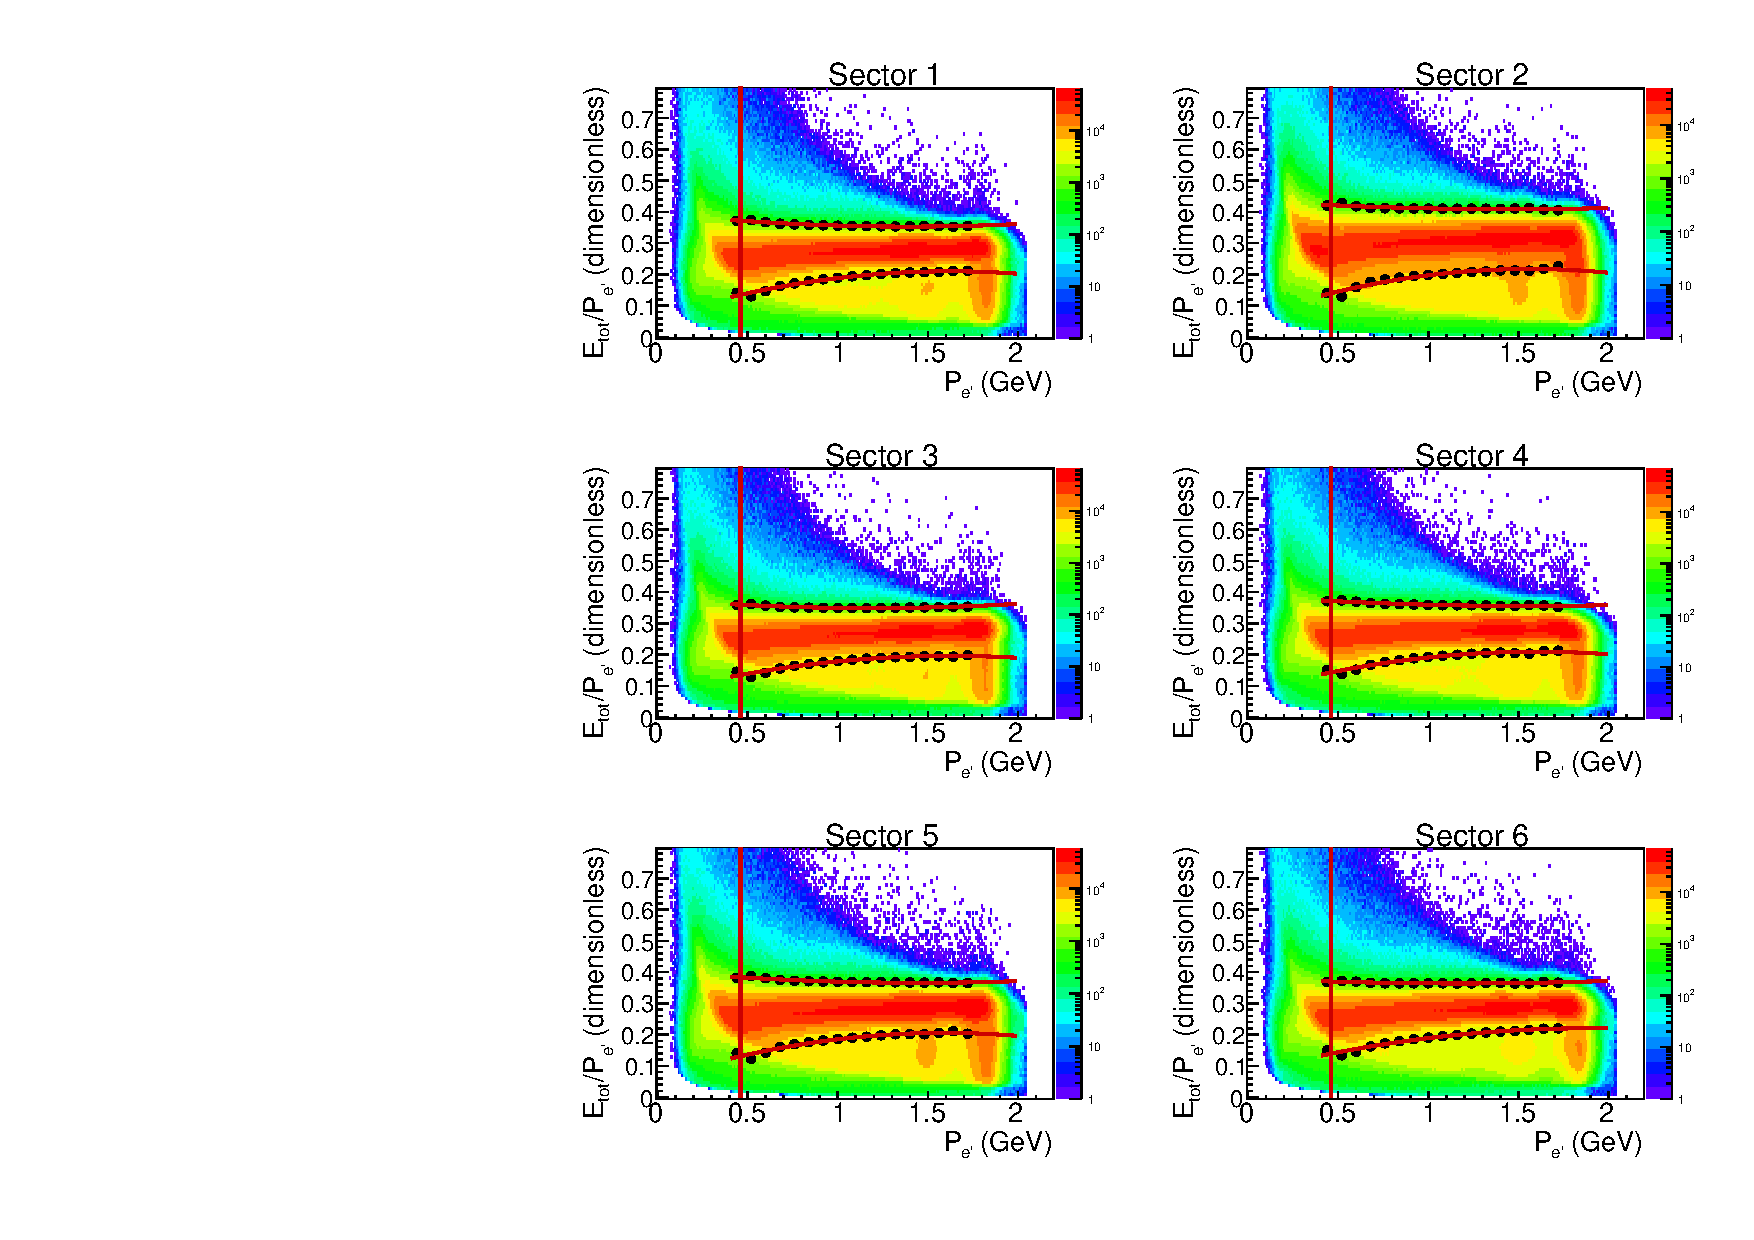
\includegraphics[width=11cm]{pictures/event_selection/ec_cut/ectot_cut_data.pdf}}
\caption{\small Sampling fraction distributions for the data. The six plots correspond to the six CLAS sectors. The vertical red line at $P_{e'} = 0.461$~GeV shows the EC threshold cut. Black points correspond to the positions of Gaussian fit maxima $\pm 3\sigma$ for different $X$-slices of the 2D histograms. These points are fit by a second order polynomial, the resulting functions are shown by the red curves. Events between the red curves are selected for further analysis.} \label{fig:ec_cut_data}
\end{center}
\end{figure}

\begin{figure}[htp]
\begin{center}
\framebox{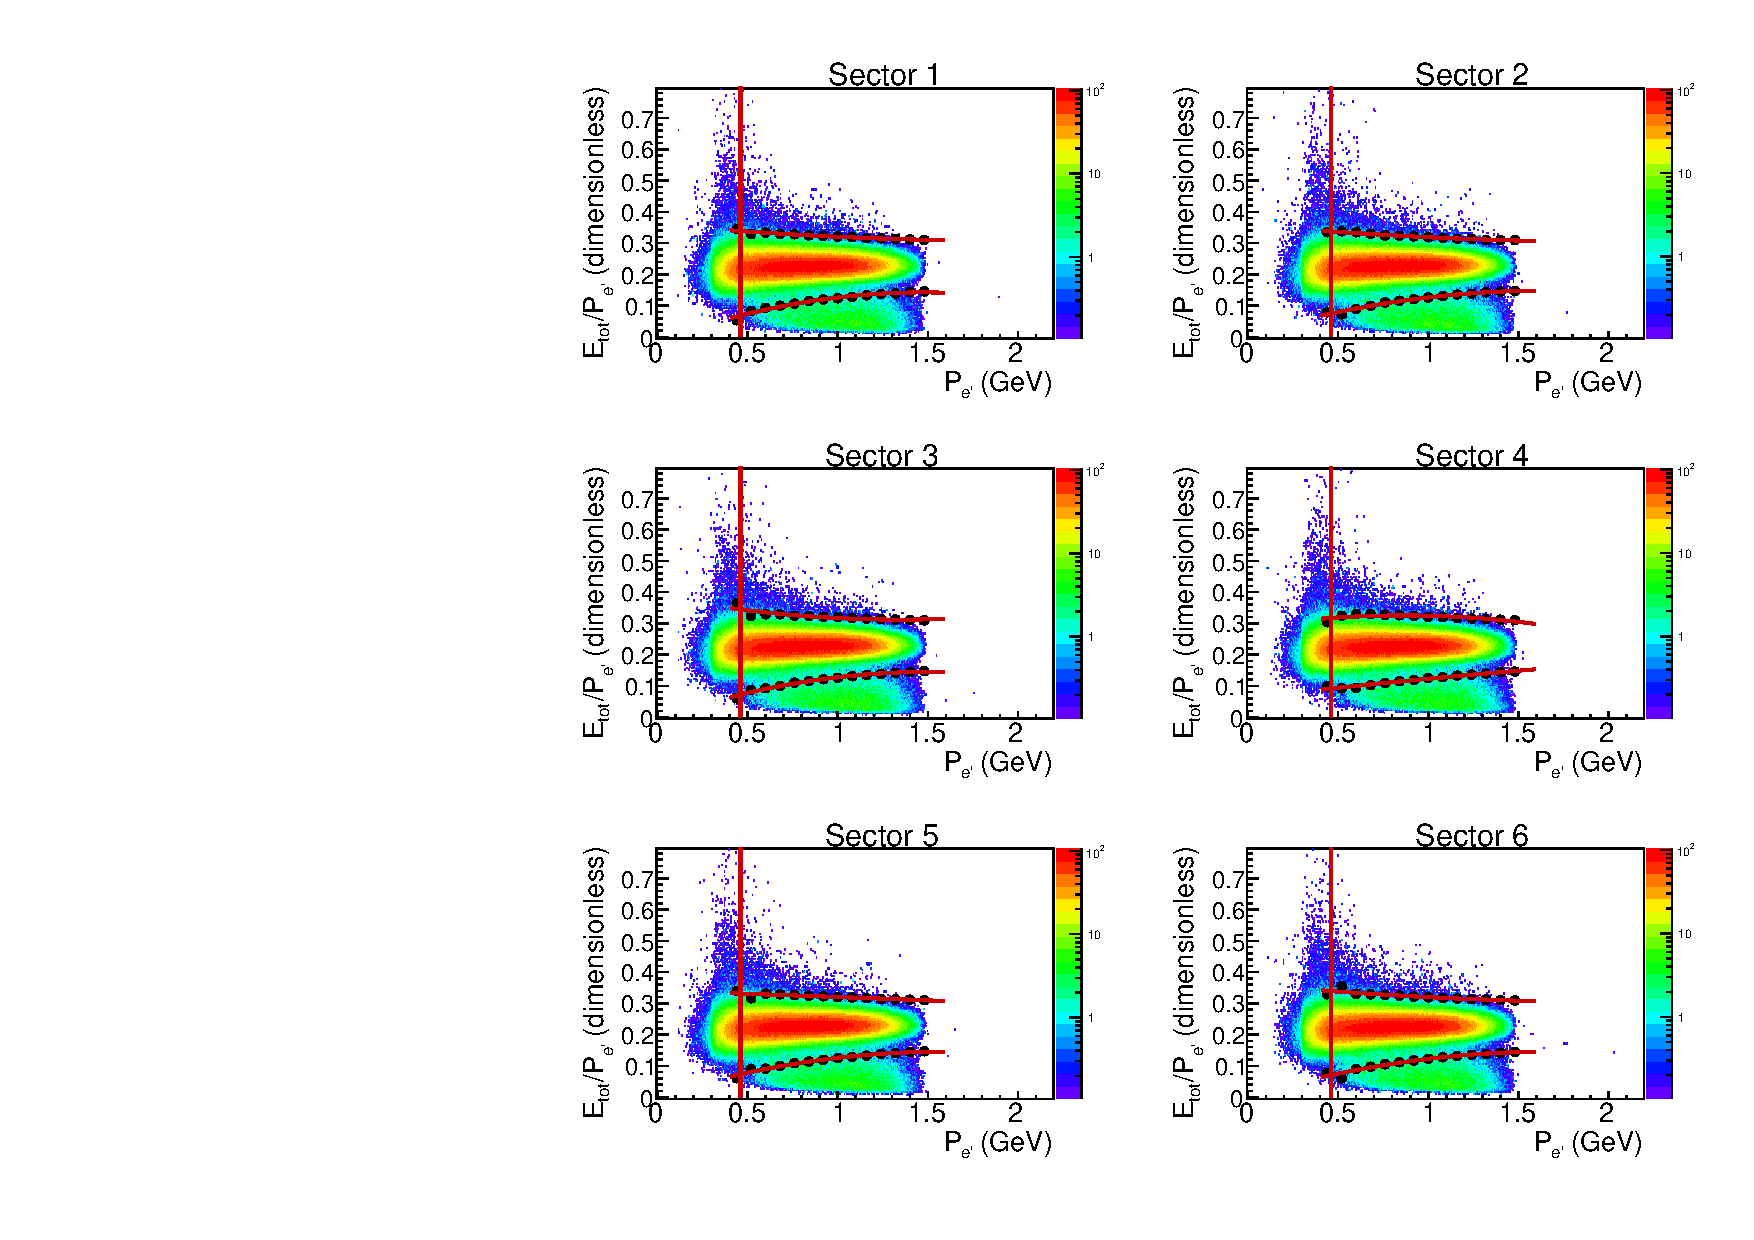
\includegraphics[width=11cm]{pictures/event_selection/ec_cut/ectot_cut_sim.pdf}}
\caption{\small  Sampling fraction distributions for the reconstructed Monte Carlo events. The six plots correspond to the six CLAS sectors. The vertical red line at $P_{e'} = 0.461$~GeV shows the EC threshold cut. Black points correspond to the positions of Gaussian fit maxima $\pm 3\sigma$ for different $X$-slices of the 2D histograms. These points are fit by a second order polynomial, the resulting functions are shown by the red curves. Events between red curves are selected for further analysis.} \label{fig:ec_cut_sim}
\end{center}
\end{figure}


Then, the so-called sampling fraction cut is applied to eliminate part of the pion contamination. To develop this cut, the fact that electrons and pions have different energy deposition patterns in the EC is used. An electron produces an electromagnetic shower, where the deposited energy $E_{tot}$ is proportional to the scattered electron momentum $P_{e'}$, while a $\pi^{-}$ loses a constant amount of energy per scintillator ($\sim$2~MeV/cm) independently of its momentum. Therefore, for electrons the quantity $E_{tot}/P_{e'}$ plotted as a function of $P_{e'}$ should follow the straight line that is parallel to the $x$-axis and located around the value 1/3 on the $y$-axis, since electrons lose about 2/3 of their energy in lead sheets (in reality this line has a slight slope).


In Fig.~\ref{fig:ec_cut_data} the total energy deposited in the EC divided by the particle momentum is shown as a function of particle momentum. The six plots correspond to the six CLAS sectors. Events between the red curves are selected as good electron candidates for further analysis. The vertical red line at $P_{e'} = 0.461$~GeV shows the EC threshold cut. The upper and lower red curves are obtained in the following way:  $X$-slices of the 2D histograms are fit by Gaussians. In this way points that correspond to the positions of the fit maxima $\pm 3\sigma$ are obtained. These points are shown by black circles in Fig.~\ref{fig:ec_cut_data}. They determine the upper and lower boundaries for the cut. Finally, to obtain smooth curves, all points are fit by a second order polynomial.  


Cuts on the minimal electron momentum and on sampling fraction are applied both to the experimental and reconstructed Monte Carlo events. Since the Monte Carlo simulation does not reproduce electromagnetic showers well enough, the sampling fraction distributions for the simulation are slightly lower than for the data. EC cuts for the simulation, obtained using the same  procedure as for the data, are shown in Fig.~\ref{fig:ec_cut_sim}. These plots contain no events with $P_{e'} > 1.5$~GeV since only double-pion events were generated, while for the data events with $P_{e'} > 1.5$~GeV exist since Figure~\ref{fig:ec_cut_data} was plotted for inclusive electrons.



\subsection{Electron selection in the CC}
\label{Sect:cc_cuts} 
To improve the quality of the electron candidate selection and $\pi^{-}/e^{-}$ separation, a \v Cerenkov counter is used~\cite{Adams:2001kk}. As shown in~\cite{Osipenko:2004}, there is a contamination in the measured CC spectra that manifests itself as a so-called single-photoelectron peak, which is actually located at a few photoelectrons (see the distributions shown in black in Fig.~\ref{fig:nphe_all_seg}). The main source of this contamination are accidental coincidences of PMT noise signals with measured pion tracks~\cite{Osipenko:2004}. The goal of CC cuts is to separate the spectrum of good electron candidates (it corresponds to the main maximum of the photoelectron distribution) from the single-photoelectron peak, but at the same time to minimize the loss of good events. As seen in Fig.~\ref{fig:nphe_all_seg} (black curves), where photoelectron distributions are plotted, the single-photoelectron peak is rather pronounced and it significantly overlaps with the spectrum of good electron candidates. Thus the elimination of this contamination is not a straightforward task and a special procedure has been developed for this purpose. 

The following set of CC cuts was applied:%\vspace{-0.5em}
\begin{itemize}
\item fiducial cut,\vspace{-0.5em}
\item $\varphi_{cc}$ matching cut,\vspace{-0.5em}
\item $\theta_{cc}$ matching cut,\vspace{-0.5em}
\item geometrical cut that removes inefficient zones, and\vspace{-0.5em}
\item standard procedure of dealing with the single-photoelectron peak contamination based on the fit of the photoelectron distributions by the modified Poisson function.
\end{itemize}

All these cuts, except the last one, are defined in the so-called ``CC projective plane"~\cite{Osipenko:2004}. This is an imaginary plane behind the CC where the \v Cerenkov radiation would arrive if its polygonal (due to reflections in the mirror system) path from the emission point to the PMT was substituted by a straight line preserving the initial propagation direction and the total distance traveled~\cite{Osipenko:2004,Adams:2001kk}. The polar and azimuthal angles $(\theta_{cc},\varphi_{cc})$, which are defined in this projective plane, are not directly available in the BOS banks~\cite{BOS:bank}. Therefore, some calculations are made to derive these angles from the variables available in the DCPB bank. Figure~\ref{fig:cc_plane_def} illustrates these calculations.


The CC projective plane is defined in the sector reference coordinate system, i.e. the sector is bisected in the middle by the $xz$-plane with the $z$-axis directed along the beam line. In this reference system the equation of the projective plane is the following (according to Ref.~\cite{Osipenko:2004}),\newpage
\begin{equation}
\begin{aligned}
 &Ax+By+Cz+D = 0,  \\ \label{eq:cc_plane}
 &A=-0.000785,~~B=0,  \\
 &C=-0.00168,~~~D=1,  \\
 &\overrightarrow{S} = (A,B,C),
\end{aligned}  
\end{equation}
where $\overrightarrow{S}$ is a vector perpendicular to the projective plane.


In Fig.~\ref{fig:cc_plane_def} the particle track in the DC is shown by the thin dashed curve. Since the particle moves through a magnetic field in the DC, the track is curved. Having left the magnetic field region of the DC, the particle moves further along a straight line, tangential to a curved DC track in the point of its intersection with the CC. The unit vector that defines the direction of this tangent is known from the DCPB bank $ \overrightarrow{n} = (n_{x}, n_{y}, n_{z}) = ($CX\_SC,~CY\_SC,~CZ\_SC$)$. In Fig.~\ref{fig:cc_plane_def} the vector $ \overrightarrow{t}$ is pointing this direction and goes from the SC hit point to the CC projective plane.


\begin{figure}[htp]
\begin{center}
\framebox{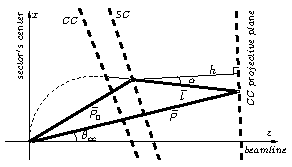
\includegraphics[width=13.5cm]{pictures/event_selection/cc_cut/cc_plane_def_new.pdf}}
\caption{\small  Illustration for the calculation of the polar $\theta_{cc}$ and azimuthal $\varphi_{cc}$ angles in the CC projective plane (see text for details).} \label{fig:cc_plane_def}
\end{center}
\end{figure}


The $(\theta_{cc},\varphi_{cc})$ angles in the projective plane are determined by the vector $\overrightarrow{P}=\overrightarrow{P_{0}}+\overrightarrow{t}$, where $\overrightarrow{P_{0}}$ is a vector that goes from the vertex to the point of the track intersection with the SC. Its components are known from the DCPB bank\footnote[2]{In the DCPB bank both $\overrightarrow{n}$ and $\overrightarrow{P_{0}}$ are defined in the sector reference frame.} $\overrightarrow{P_{0}} = (p_{x}^{0},p_{y}^{0},p_{z}^{0}) = ($x\_SC,~y\_SC,~z\_SC$)$.

The vector $\overrightarrow{t}$ can be defined as
\begin{equation}
 \overrightarrow{t} =  | \overrightarrow{t}  |\cdot \overrightarrow{n}  =  \frac{h}{\cos \alpha}\cdot \overrightarrow{n},
\label{eq:cc_t_vec} 
\end{equation}
where $\overrightarrow{n}$ is the unit vector in the $\overrightarrow{t}$-direction defined above, while $h$ is the distance from the SC hit point to the CC projective plane, which is given by\footnote[3]{This is a standard relation for the distance from the point (given here by the vector $\overrightarrow{P_{0}}$) to the plane $Ax+By+Cz+D = 0$. }
\begin{equation}
h=\frac{|(\overrightarrow{S} \cdot \overrightarrow{P_{0}})+D|}{ |\overrightarrow{S}  |},
\label{eq:cc_h_distance}
\end{equation}
where $\overrightarrow{S}$ is the vector normal to the CC projective plane defined by Eq.~\eqref{eq:cc_plane}.

In turn $\cos \alpha$ can be calculated as
\begin{equation}
\cos \alpha = \frac{|(\overrightarrow{S}\cdot \overrightarrow{n})|}{|\overrightarrow{S}|},
\end{equation}
since $\overrightarrow{S}$ is directed along $h$ and $\overrightarrow{n}$ is directed along $\overrightarrow{t}$. 


This leads to the following expression for the vector $\overrightarrow{t}$,
\begin{equation}
 \overrightarrow{t} =  | \overrightarrow{t}  |\cdot \overrightarrow{n}  =\left | \frac{(\overrightarrow{S} \cdot \overrightarrow{P_{0}})+D}{(\overrightarrow{S} \cdot \overrightarrow{n})}\right |\cdot \overrightarrow{n}   = \left | \frac{A\! \cdot\! p_{x}^{0}+B\! \cdot\! p_{y}^{0}+C\! \cdot\! p_{z}^{0}+D}{A \!\cdot\! n_{x}+B\! \cdot\! n_{y}+C \!\cdot\! n_{z}}\right |\cdot\overrightarrow{n}.
\label{eq:cc_t_vec} 
\end{equation}


Then, obtaining the required vector $\overrightarrow{P}$ as the sum of $\overrightarrow{P_{0}}$ and $\overrightarrow{t}$, one can finally calculate the angles $\theta_{cc}$ and $\varphi_{cc}$ as 
\begin{equation}
\begin{aligned}
\theta_{cc}&=\arccos\left ( \frac{P_z}{| \overrightarrow{P}  |}\right ),\\
\varphi_{cc} & =  \arctan\left ( \frac{P_{y}}{P_{x}} \right ). 
\label{eq:cc_phi_theta} 
\end{aligned}
\end{equation}

The angle $\varphi_{cc}$ defined by Eq.~\eqref{eq:cc_phi_theta} is determined with respect to the center of each sector. This means that $\varphi_{cc} = 0$ is the middle of the sector, $\varphi_{cc} < 0$ is on the left side of the sector, and $\varphi_{cc} > 0$ is on its right side.

One should also define the variables $CC~segment~number$ (that indicates which segment has been hit) and $index$ (that indicates which PMT has fired). They are taken from the CCPB bank $Status$ variable according to the following relation,
\begin{equation}
Status = 10\times(\text{CC segment number}) + 1000\times( 1 + index),
\label{eq:cc_segment}
\end{equation}
where $index$ is 1 for right PMTs, $-1$ for left PMTs, and 0 when both PMTs have~fired.


%---------------------------------------------------------------------------------

After all needed variables have been defined, all the cuts from the list specified above can be implemented.

First of all the fiducial cut in the CC plane is applied. The shape of this cut is taken from~\cite{Khetarpal:2010} and is given by
\begin{equation}
\begin{aligned}
\theta_{cc} > 7.0+0.0032\cdot \varphi_{cc}~+~&0.0499\cdot \varphi_{cc}^{2}, \\
\left( \frac{\theta_{cc}-45.5^{o}}{34.5^{o}} \right)^{2} + \left( \frac{\varphi_{cc}}{21^{o}} \right)^{2} &\le 1, \\
\left( \frac{\theta_{cc}-45.5^{o}}{1.75^{o}} \right)^{2} + \left( \frac{\varphi_{cc}}{21^{o}} \right)^{2} &> 1,~\textrm{and} \\
\theta_{cc} < 45^{o}. \, \, \,  \, \, \, \, \, \,   \, \, \,  \, \, \, \, \, \,
\label{eq:cc_fiduch}
\end{aligned}
\end{equation}\vspace{-1em}

Then the so-called $\varphi_{cc}$ and $\theta_{cc}$ matching procedures (based on the studies~\cite{Osipenko:2004} and~\cite{Ungaro:2010}) are performed. The idea of this matching is quite simple: there must be one-to-one correspondence between the angles in the CC plane (which are calculated based on the information from the DC) and PMT signals in the CC for real events, while background noise and accidentals should not show such correlation.

The principle of the $\varphi_{cc}$ matching cut is the following: when the track is on the right side of the CC segment, the right PMT should be fired, and vice versa. Therefore, if $\varphi_{cc}<0$, the $index$ defined in Eq.~\eqref{eq:cc_segment} is required to be $-1$ and if $\varphi_{cc}>0$, the $index$ is required to~be~1. Events that do not satisfy these conditions are removed. All events with $index=0$ are kept.

\begin{figure}[htp]
\begin{center}
\framebox{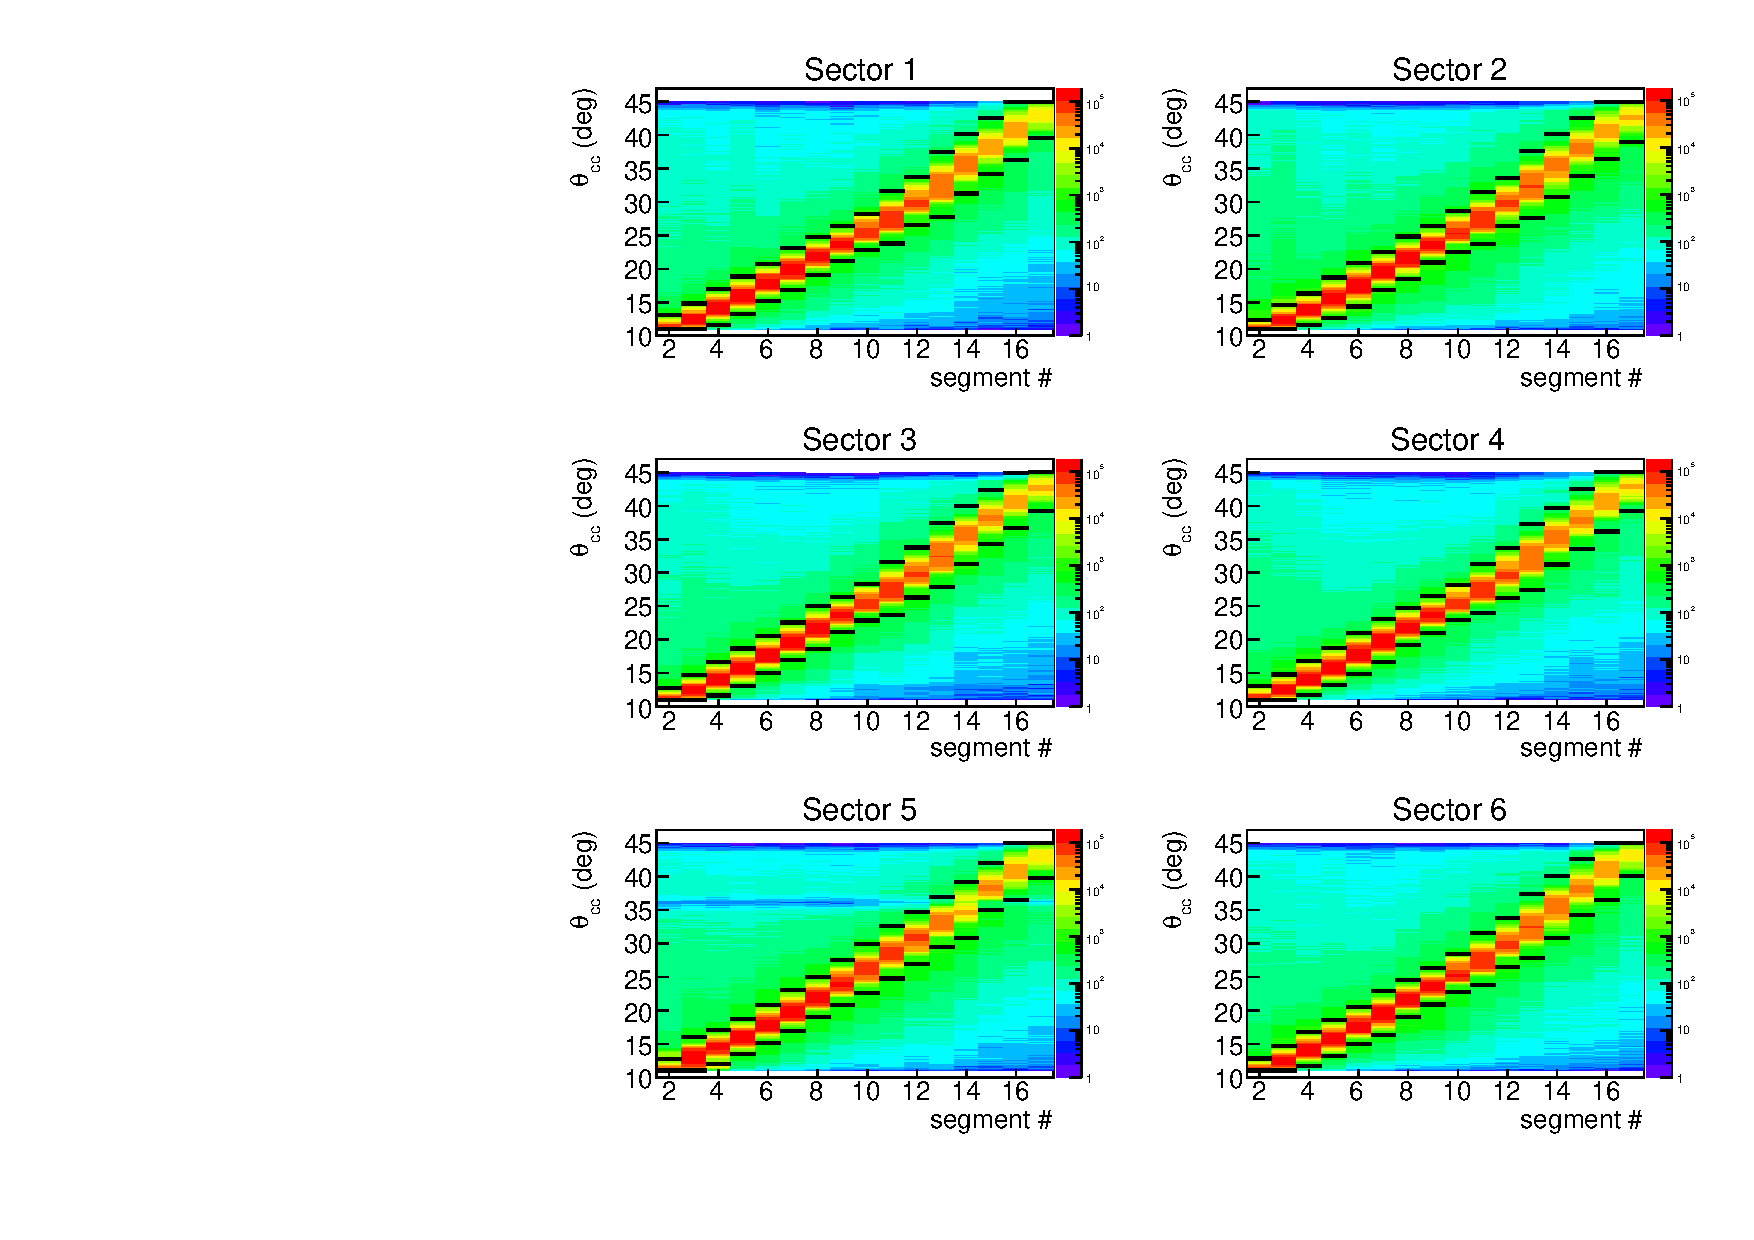
\includegraphics[width=9cm]{pictures/event_selection/cc_cut/th_vs_seg.pdf}}
\caption{\small  $\theta_{cc}$ versus segment distributions for six CLAS sectors. Events between the horizontal black lines are treated as good electron candidates.} \label{fig:th_vs_seg}
\end{center}
\end{figure}%\vspace{-1em}

In order to perform $\theta_{cc}$ matching, the $\theta_{cc}$ versus segment number cut should be done. Figure~\ref{fig:th_vs_seg} shows $\theta_{cc}$ versus segment distributions for the six CLAS sectors. Event distributions in each segment have been plotted as a function of $\theta_{cc}$ and fit by Gaussians. The horizontal black lines correspond to the positions of the fit maxima $\pm4\sigma$. Events between these black lines are treated as good electron candidates.


The influence of $\varphi_{cc}$ and $\theta_{cc}$ matching cuts on the photoelectron distributions is demonstrated in Fig.~\ref{fig:nphe_all_seg}, where the distributions before matching cuts are plotted in black, distributions after the $\varphi_{cc}$ matching are plotted in red, and after the subsequent $\theta_{cc}$ versus segment cut are plotted in blue. As seen in Fig.~\ref{fig:nphe_all_seg} both these cuts reduce the single-photoelectron peak, but leave the main part of the spectrum unchanged. The same $\varphi_{cc}$ and $\theta_{cc}$ matching cuts are also applied to the reconstructed Monte Carlo events.


The accidental noise and pion background are not the only source of the single-photoelectron peak contamination. The peak also partially corresponds to electrons that hit some specific geometrical zones with low CC efficiency. When an electron hits such a zone the number of detected photoelectrons turns out to be significantly less than expected. This leads to the fact that the region of the photoelectron spectrum, which corresponds to the low number of photoelectrons, appears to be overpopulated by events. Since low efficiency zones are distributed inhomogeneously in the CC plane and the Monte Carlo simulation do not reproduce them properly, it is better to remove them from the consideration completely. For this purpose  a special geometrical cut is established. 


This geometrical cut is done in the following way. Distributions $\varphi_{cc}$ versus $\theta_{cc}$ are plotted for each CLAS sector (see Fig.~\ref{fig:ph_vs_th_cc}, upper frame) with the quantity~\eqref{eq:cc_ratio} as a color code. 
\begin{equation}
\frac{number\,\, of\,\, events\,\,  inside\,\, (\theta_{cc},\varphi_{cc})\,\, bin\,\, with\,\, more\,\, than\,\, five\,\, photoelectrons }{total\,\, number\,\, of\,\, events\,\,  inside\,\, (\theta_{cc},\varphi_{cc})\,\, bin}
\label{eq:cc_ratio}
\end{equation}%\vspace{-1em}

This quantity varies from zero to one and shows the proportion of electron candidates with number of photoelectrons greater than five inside a $(\theta_{cc},\varphi_{cc})$ bin. The value for this criterion (five photoelectrons) was chosen rather arbitrarily, since its only purpose is to facilitate the separation of inefficient zones (which correspond mostly to low numbers of photoelectrons) from the regular zones (which correspond to the full photoelectron spectrum). 

The curved vertical stripe in sector five in Fig.~\ref{fig:ph_vs_th_cc} corresponds to an inefficient zone that will be discussed further in~Sect.~\ref{Sect:fiduc_neg}.

\begin{figure}[htp]
\begin{center}
\framebox{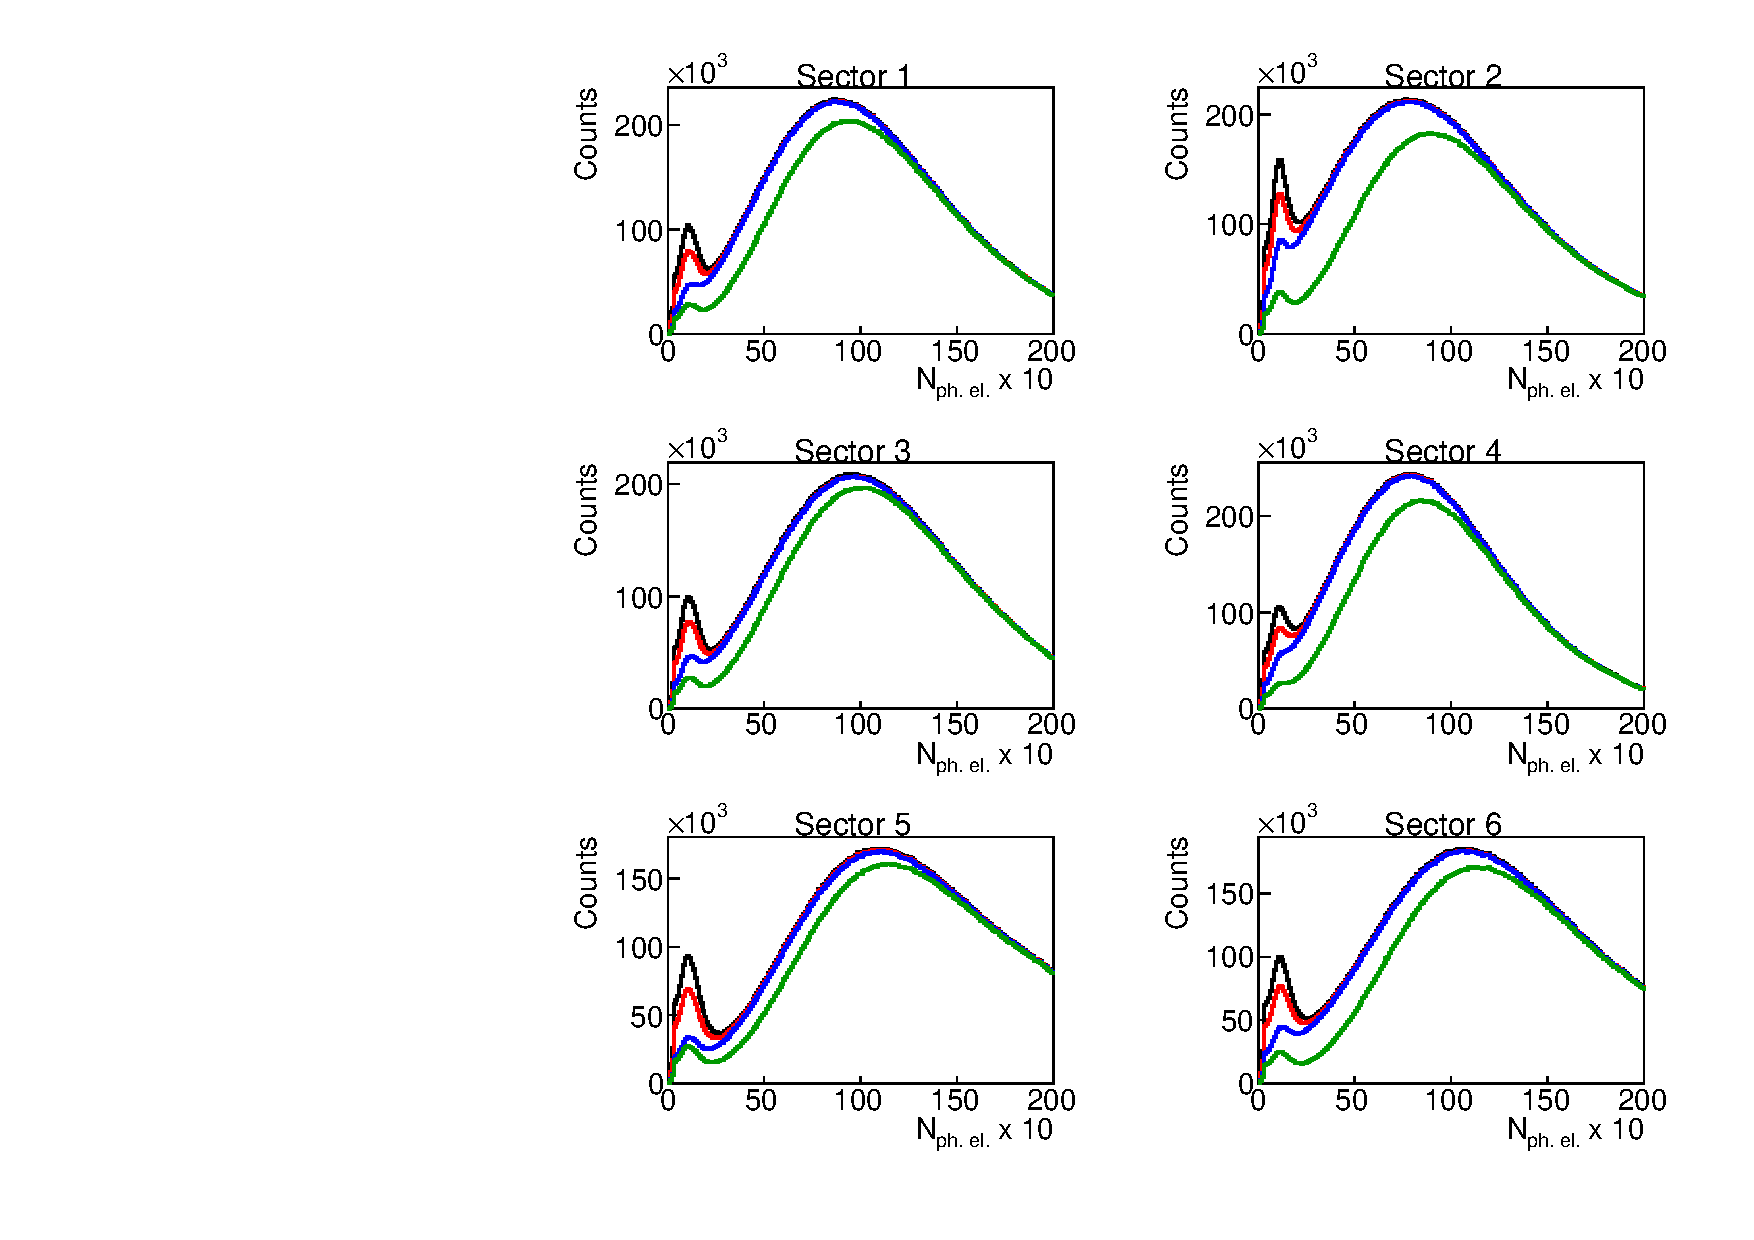
\includegraphics[width=9cm]{pictures/event_selection/cc_cut/nphe_all_seg_bef_aft_diff_cuts.pdf}}
\caption{\small Influence of different CC cuts on the distributions of the number of photoelectrons multiplied by ten for the six CLAS sectors. Black curve -- only fiducial cut in the CC plane is applied, red curve -- the $\varphi_{cc}$ matching cut is added, blue curve -- the $\theta_{cc}$ matching cut is added, and green curve -- the geometrical cut in the CC plane that removes inefficient zones is finally added.} \label{fig:nphe_all_seg}
\end{center}
\end{figure}

For further analysis only fiducial areas with a ratio~\eqref{eq:cc_ratio} greater than the certain threshold value are selected. This threshold value was chosen to be 0.7, 0.65, 0.7, 0.65, 0.8, and 0.8 for sectors 1, 2, 3, 4, 5, and 6, respectively. Since inefficient zones are not identical for various CLAS sectors (see Fig.~\ref{fig:ph_vs_th_cc}), different threshold values are needed for them. Geometrical zones, which are selected for further analysis, are shown in black in the lower plots of Fig.~\ref{fig:ph_vs_th_cc}. All zones shown in white are treated as inefficient and are removed from the analysis. As seen in Fig.~\ref{fig:ph_vs_th_cc}, there is an inefficient zone in the middle of each sector. This is expected since two CC mirrors are joined here. 

\begin{figure}[htp]
\begin{center}
\framebox{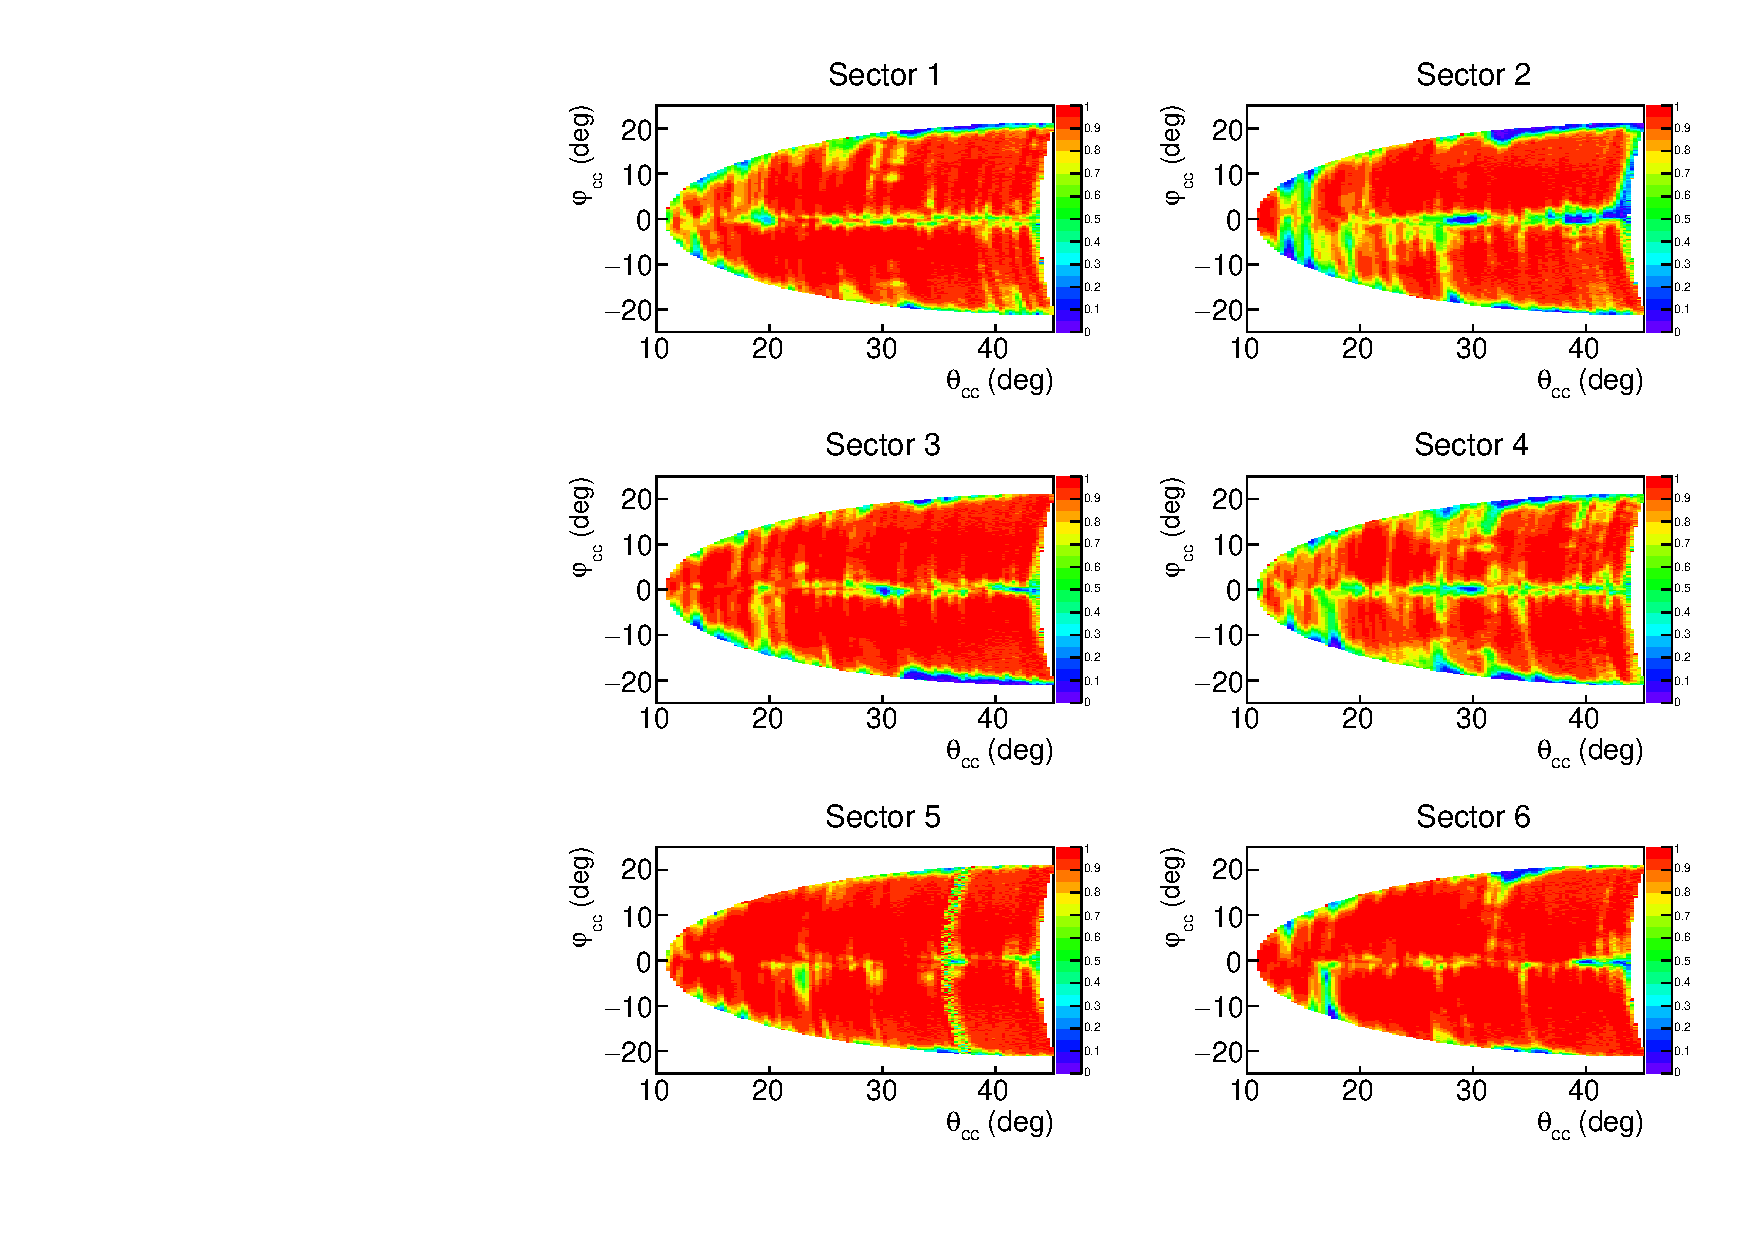
\includegraphics[width=9cm]{pictures/event_selection/cc_cut/cc_2dim_hists_div.pdf}}
\framebox{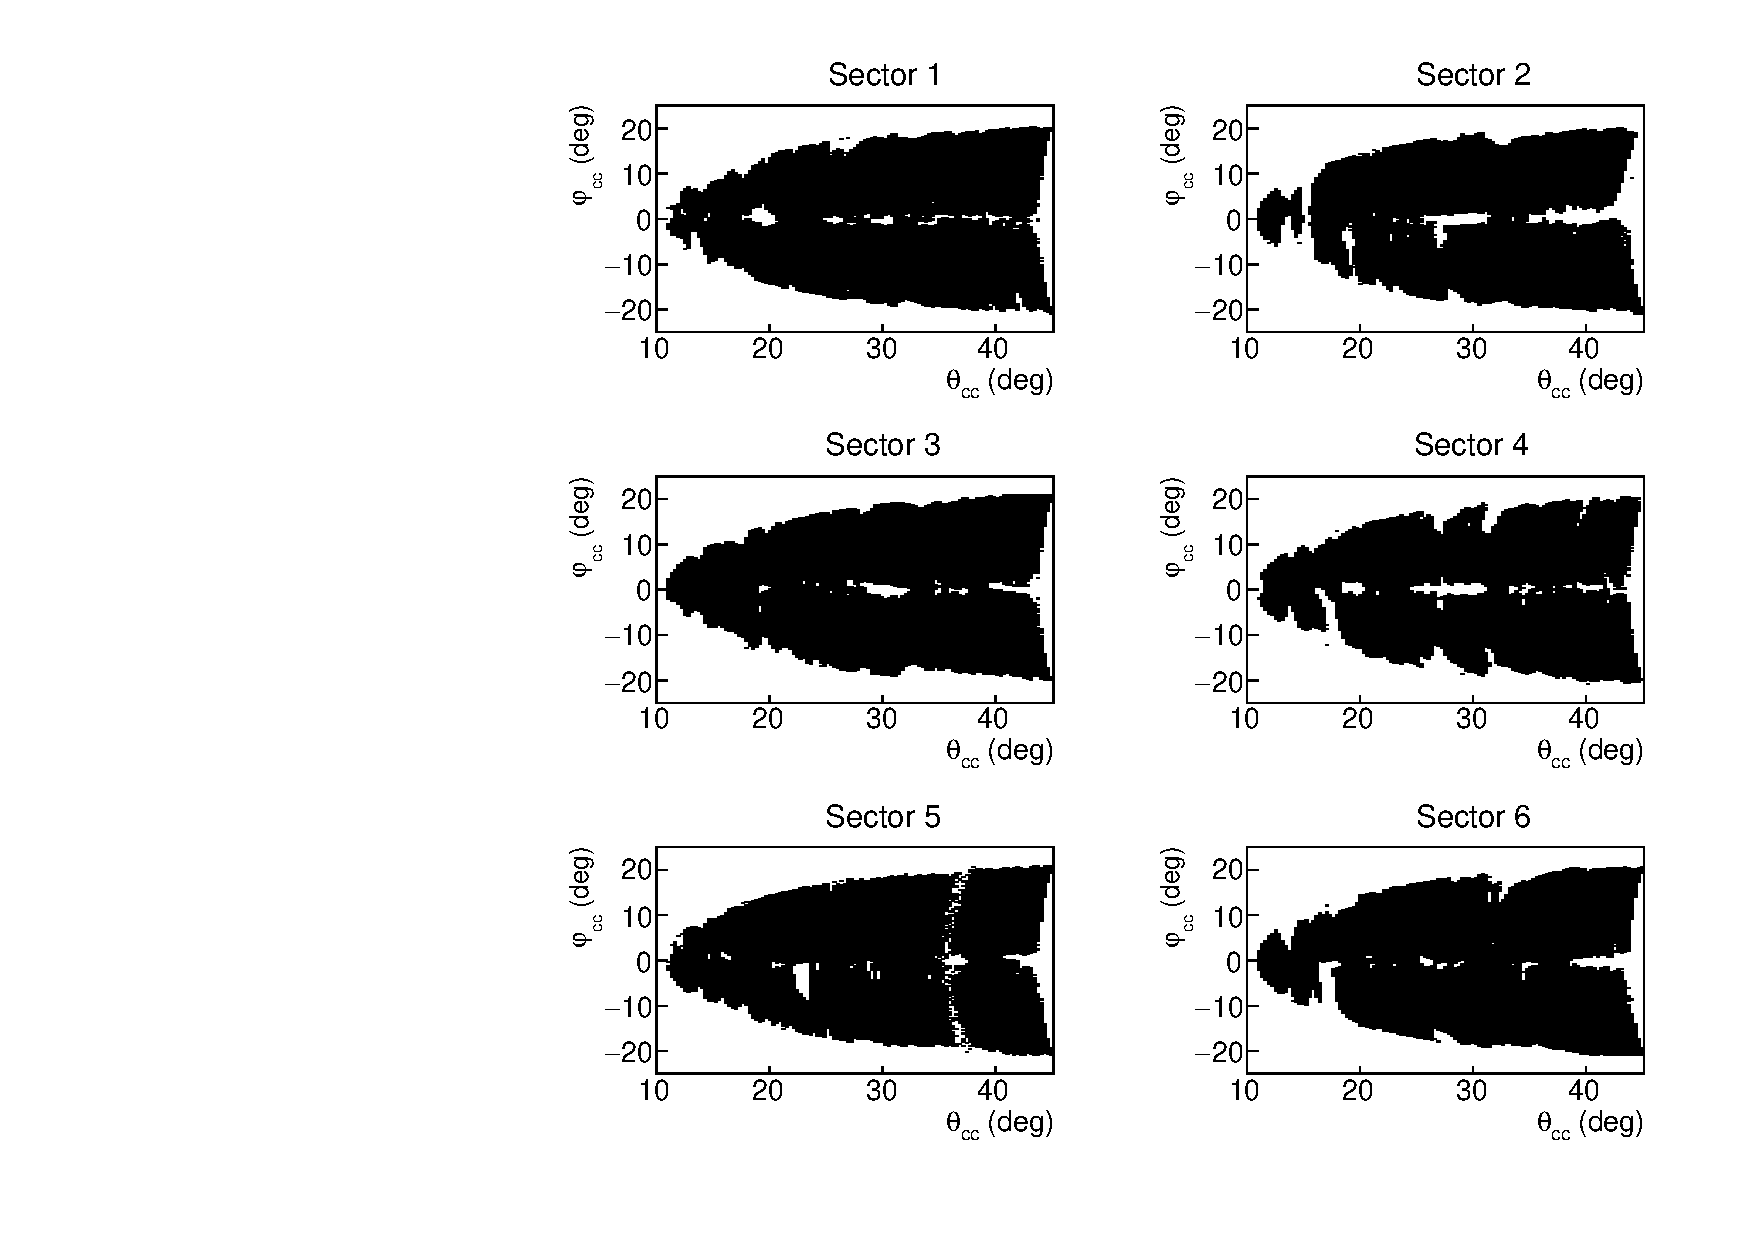
\includegraphics[width=9cm]{pictures/event_selection/cc_cut/cc_geom_cut_gt_065_07_08.pdf}}
\caption{\small Upper frame: Distributions of the quantity~\eqref{eq:cc_ratio} as a function of the polar $\theta_{cc}$ and azimuthal $\varphi_{cc}$ angles in the CC plane for the six CLAS sectors. This quantity varies from zero to one and shows the proportion of electron candidates with number of photoelectrons greater than five inside a $(\theta_{cc},\varphi_{cc})$ bin. Lower frame: Black zones correspond to the fiducial areas with the ratio~\eqref{eq:cc_ratio} greater than 0.7, 0.65, 0.7, 0.65, 0.8, and 0.8 for sectors 1, 2, 3, 4, 5, and 6, respectively. These zones are selected for further analysis. All zones shown in white are treated as inefficient and removed from the analysis.} \label{fig:ph_vs_th_cc}
\end{center}
\end{figure}

The threshold values for the ratio~\eqref{eq:cc_ratio} were chosen in order to keep the balance between the intention to reduce the amount of low efficient zones as much as possible and the desire to preserve most of the statistics. The influence of this geometrical cut on the photoelectron distributions in different sectors is demonstrated in Fig.~\ref{fig:nphe_all_seg}, where the distributions after the cut are plotted in green. As was expected, this cut leads to some reduction in the low lying part of the photoelectron spectrum, including the region of the single-photoelectron peak, and leaves the high lying part of the spectrum unchanged.


This geometrical cut is fully based on the experimental data. It acts as a fiducial cut, because it simply removes certain geometrical regions in the CC plane. This means that it can be safely applied to the Monte Carlo simulation, too. Thus, the same geometrical regions (shown in white in the lower plots in Fig.~\ref{fig:ph_vs_th_cc}) are removed both for the experimental and reconstructed Monte Carlo events.


After the geometrical cut discussed above is applied, the single-photoelectron peak appears to be significantly smaller and better separated from the main spectrum, but still remains (see Fig.~\ref{fig:nphe_all_seg}). Therefore, in order to completely get rid of this contamination, the standard procedure should then be applied~\cite{Fed_an_note:2007}. 


To apply the standard procedure of dealing with the single-photoelectron peak contamination, the photoelectron distributions are plotted for each PMT on the left and right sides of each CC segment and for each CLAS sector (see Fig.~\ref{fig:nphe_cut}). 


In Fig.~\ref{fig:nphe_cut} the red lines show the cuts that are made in order to eliminate events under the single-photoelectron peak. The cut position is individually optimized for each PMT in each sector. The distributions of events, for which both right and left PMTs have fired ($index = 0$) are not subject to this cut, since their contamination caused by the single-photoelectron peak is assumed negligible.


Since the Monte Carlo does not reproduce photoelectron distributions well enough, the cut shown by the red lines in Fig.~\ref{fig:nphe_cut} is applied only to the data. To recover the good electrons that were cut off in this way, a special procedure is applied. The part of the distributions on the right side of the red line is fit by the function~\eqref{eq:cc_Poisson}, which is a slightly modified Poisson distribution. 
\begin{equation}
y = P_{1}\left(\frac{P_{3}^{\frac{x}{P_{2}}}}{\Gamma\left(\frac{x}{P_{2}}+1\right)}
\right)e^{-P_{3}},
\label{eq:cc_Poisson}
\end{equation}
where $P_{1}$, $P_{2}$, and $P_{3}$ are free fit parameters.

\begin{figure}[htp]
\begin{center}
\framebox{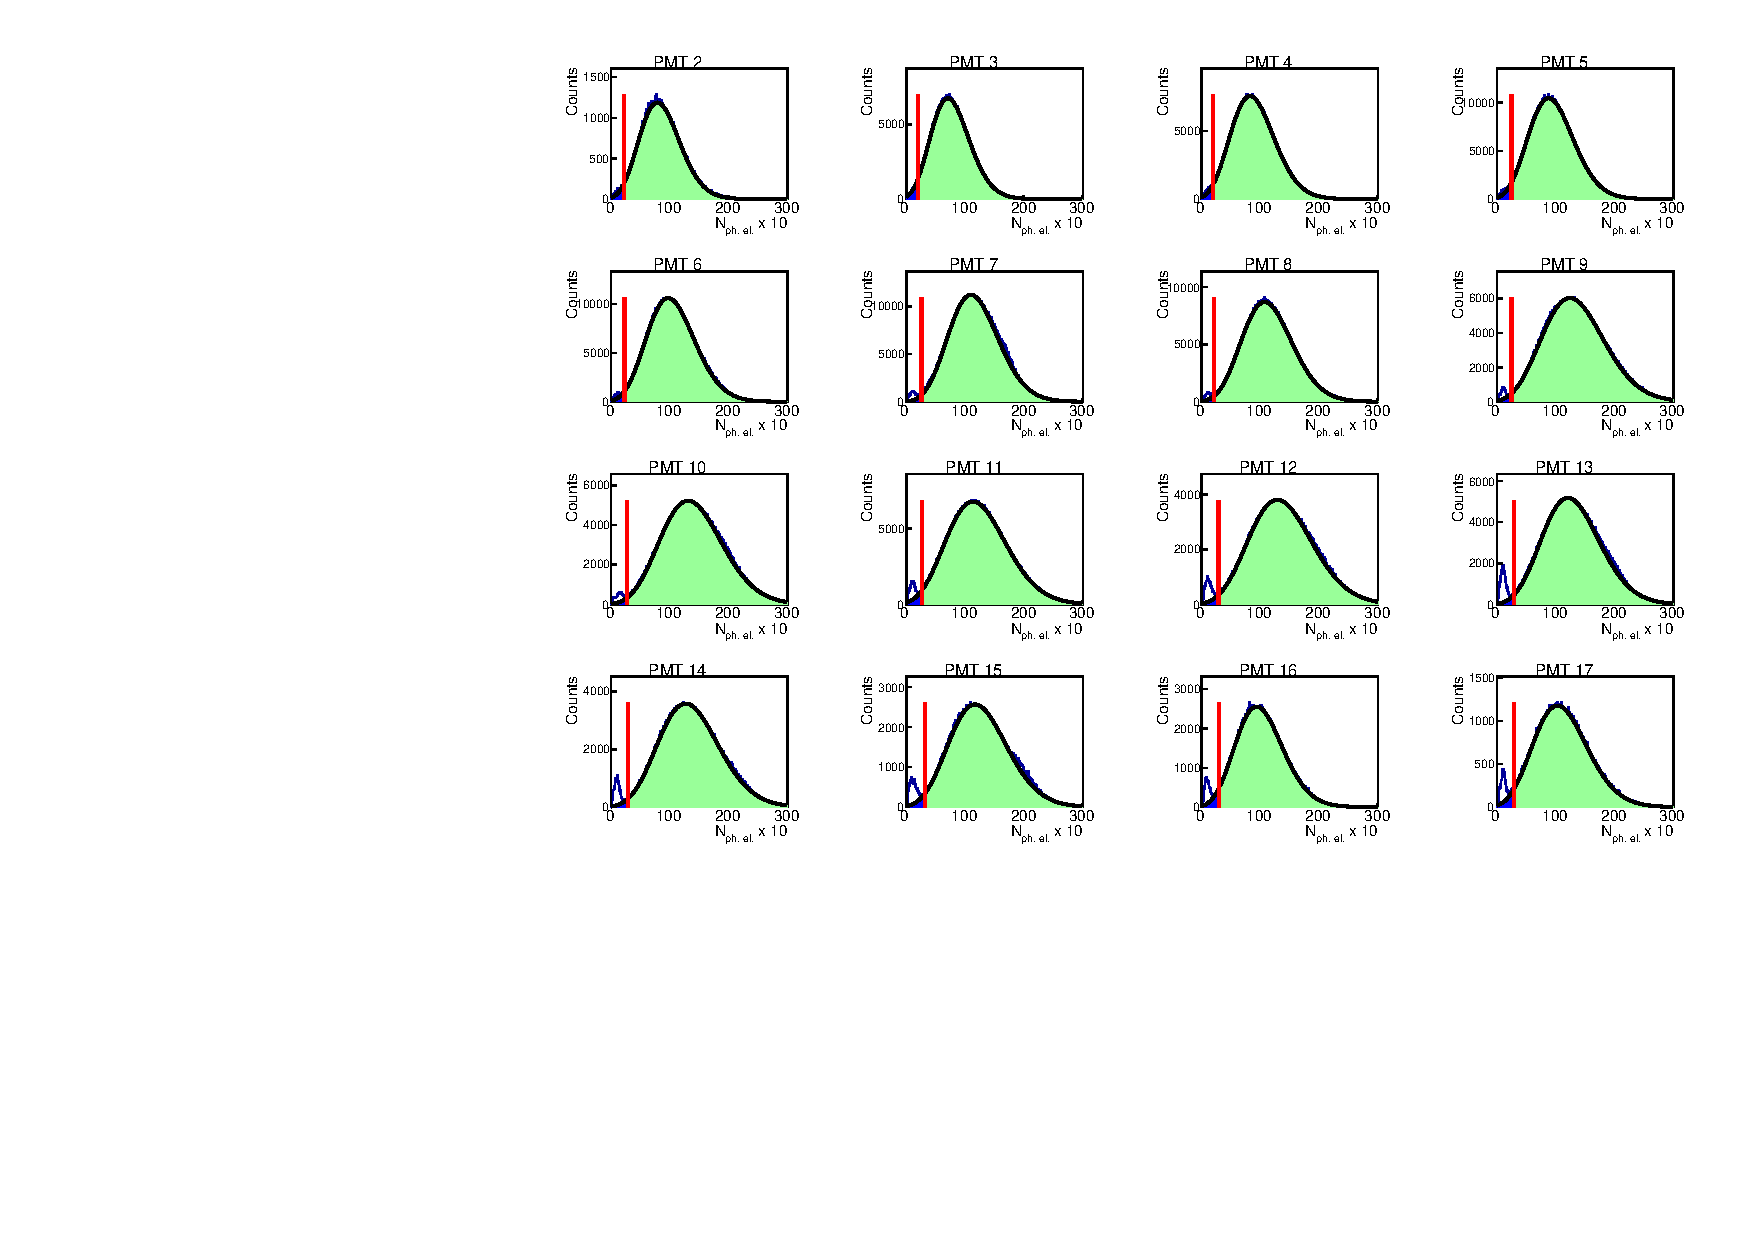
\includegraphics[width=15cm]{pictures/event_selection/cc_cut/ph_el_cut_s1_left_new.pdf}}
\caption{\small Distributions of number of photoelectrons multiplied by ten for the left side of sector one of the CC. Various plots correspond to various CC segments. Black curves show the fit by the function~\eqref{eq:cc_Poisson}. Red vertical lines show the applied cut. Regions that are needed to calculate the correction ratio~\eqref{eq:cc_corr_fact} are shown in blue and green. } \label{fig:nphe_cut}
\end{center}
\end{figure}


The fitting function is then continued into the region on the left side of the red line. In this way the two regions, shown in blue and green in Fig.~\ref{fig:nphe_cut}, are determined. Finally the correction factors are defined by~\eqref{eq:cc_corr_fact} and applied as a weight for each event, which goes to the particular PMT. These correction factors depend on the PMT number and are typically on a level of a few percent.
\begin{equation}
F_{ph.\,\, el.} = \frac{\textrm{green\,\,  area \,\,+\,\, blue\,\,  area}}{\textrm{green\,\,  area}}
\label{eq:cc_corr_fact}
\end{equation}

Note that segments \#1 and \#18 are removed from the analysis completely (both in data and Monte Carlo), since they are dominated by events from the single-photoelectron peak. 


%-------------------------------------------


\section{Hadron identification}
\label{Sect:hadr_id}
%The CLAS TOF system provides information,
% ($\beta_{h} =\frac{v_{h}}{c}$). In this analysis the value of $\beta_{h}$ was derived as the following:
Hadron are identified relying on the information provided by the TOF system~\cite{Smith:1999ii, clas_tof_paddles}. This information allows the velocity of the hadron candidates to be determined according to the following relation.
\begin{equation}
\beta_{h} =\frac{v_{h}}{c}=\frac{l_{h}}{t_{h}\cdot c},
\label{eq:beta_new}
\end{equation}
where $v_{h}$ is the hadron velocity, $c$ the speed of light, $l_{h}$ the hadron path length from the vertex to the SC-plane (variable \textit{Path} in the SCPB bank), and $t_{h}$ the time that it took the hadron to travel from the vertex to the SC-plane. This time can be calculated in the following way. 
\begin{equation}
t_{h} = t_{e} + (t^{tof}_{h}- t^{tof}_{e}) = \frac{l_{e}}{c} + (t^{tof}_{h}- t^{tof}_{e})  ,
\label{eq:time_hadron}
\end{equation}
where $t_{e} = \frac{l_{e}}{c}$ is the time that the electron spent on traveling from the vertex to the SC-plane and $l_{e}$ the electron path length. The quantities $t^{tof}_{e}$ and $t^{tof}_{h}$ are the times, when the electron and hadron hit the SC-plane, respectively (the variable \textit{Time} in the SCPB bank).

Equation~\eqref{eq:time_hadron} assumes that the hadron and electron departed from the vertex at the same time, but the electron traveling with the speed of light reached the SC-plane earlier than the hadron. The difference $t^{tof}_{h} - t^{tof}_{e}$ indicates the hadron delay time, which is the consequence of traveling with the velocity $v_{h}<c$. Thus Eq.~\eqref{eq:time_hadron} makes the hadron time related to that of electron for each event\footnote[4]{It worth noting that usually one uses the value of $\beta$ directly defined in the EVNT bank (variable \textit{Betta}), but it turned out that this quantity shows noticeable inaccuracies in electron bunch determination, which were made during the cooking. The value of $\beta$ calculated by Eqs.~\eqref{eq:beta_new} and ~\eqref{eq:time_hadron} do not show these inaccuracies because in this method the timing of the hadron is related to that of electron for each event. }.  

The charged hadron can be identified by comparing $\beta_{h}$ determined from TOF according to Eqs.~\eqref{eq:beta_new} and ~\eqref{eq:time_hadron} with $\beta_{n}$ given by 
\begin{equation}
\beta_{n}=\frac{p_{h}}{\sqrt{p_{h}^{2}+m_{h}^{2}}}.
\label{eq:hadron_hadronmass}
\end{equation}

In Eq.~\eqref{eq:hadron_hadronmass} $\beta_{n}$ is a so-called nominal value that is calculated using the particle momentum ($p_{h}$) known from the DC and the exact particle mass assumption ($m_{h}$).

The usual way to develop hadron id cuts is to investigate $\beta$ versus momentum distributions for different TOF paddles for each hadron type separately. This investigation reveals three types of problematic paddles, i.e.

\begin{enumerate}[label=\Alph*]\vspace{-0.5em}
\item  Paddles which signals are completely unreliable (bad paddles). These are paddles \#16 in sector 2, \#44 in sector 3, \#17 in sector 5, and \#48 in each sector. They are excluded from this analysis both for experimental data and reconstructed Monte Carlo events. 
\item Paddles in which the distributions are shifted from their expected positions. The reason for this is most likely mistakes during data cooking/calibration. Typical examples of such paddles are shown in Fig.~\ref{fig:shifted_paddles}.
\item Paddles for which the distributions for a given hadron have double band structure. This problem appears for most of the paddles with number $\geq 40$ and originates from the fact that (along with the mistakes during cooking/calibration) for these paddles two scintillation bars were connected to one TDC~\cite{clas_tof_paddles}. Typical examples of such paddles are shown in Fig.~\ref{fig:double_paddles}.
\end{enumerate}

\begin{figure}[htp]
\begin{center}
\framebox{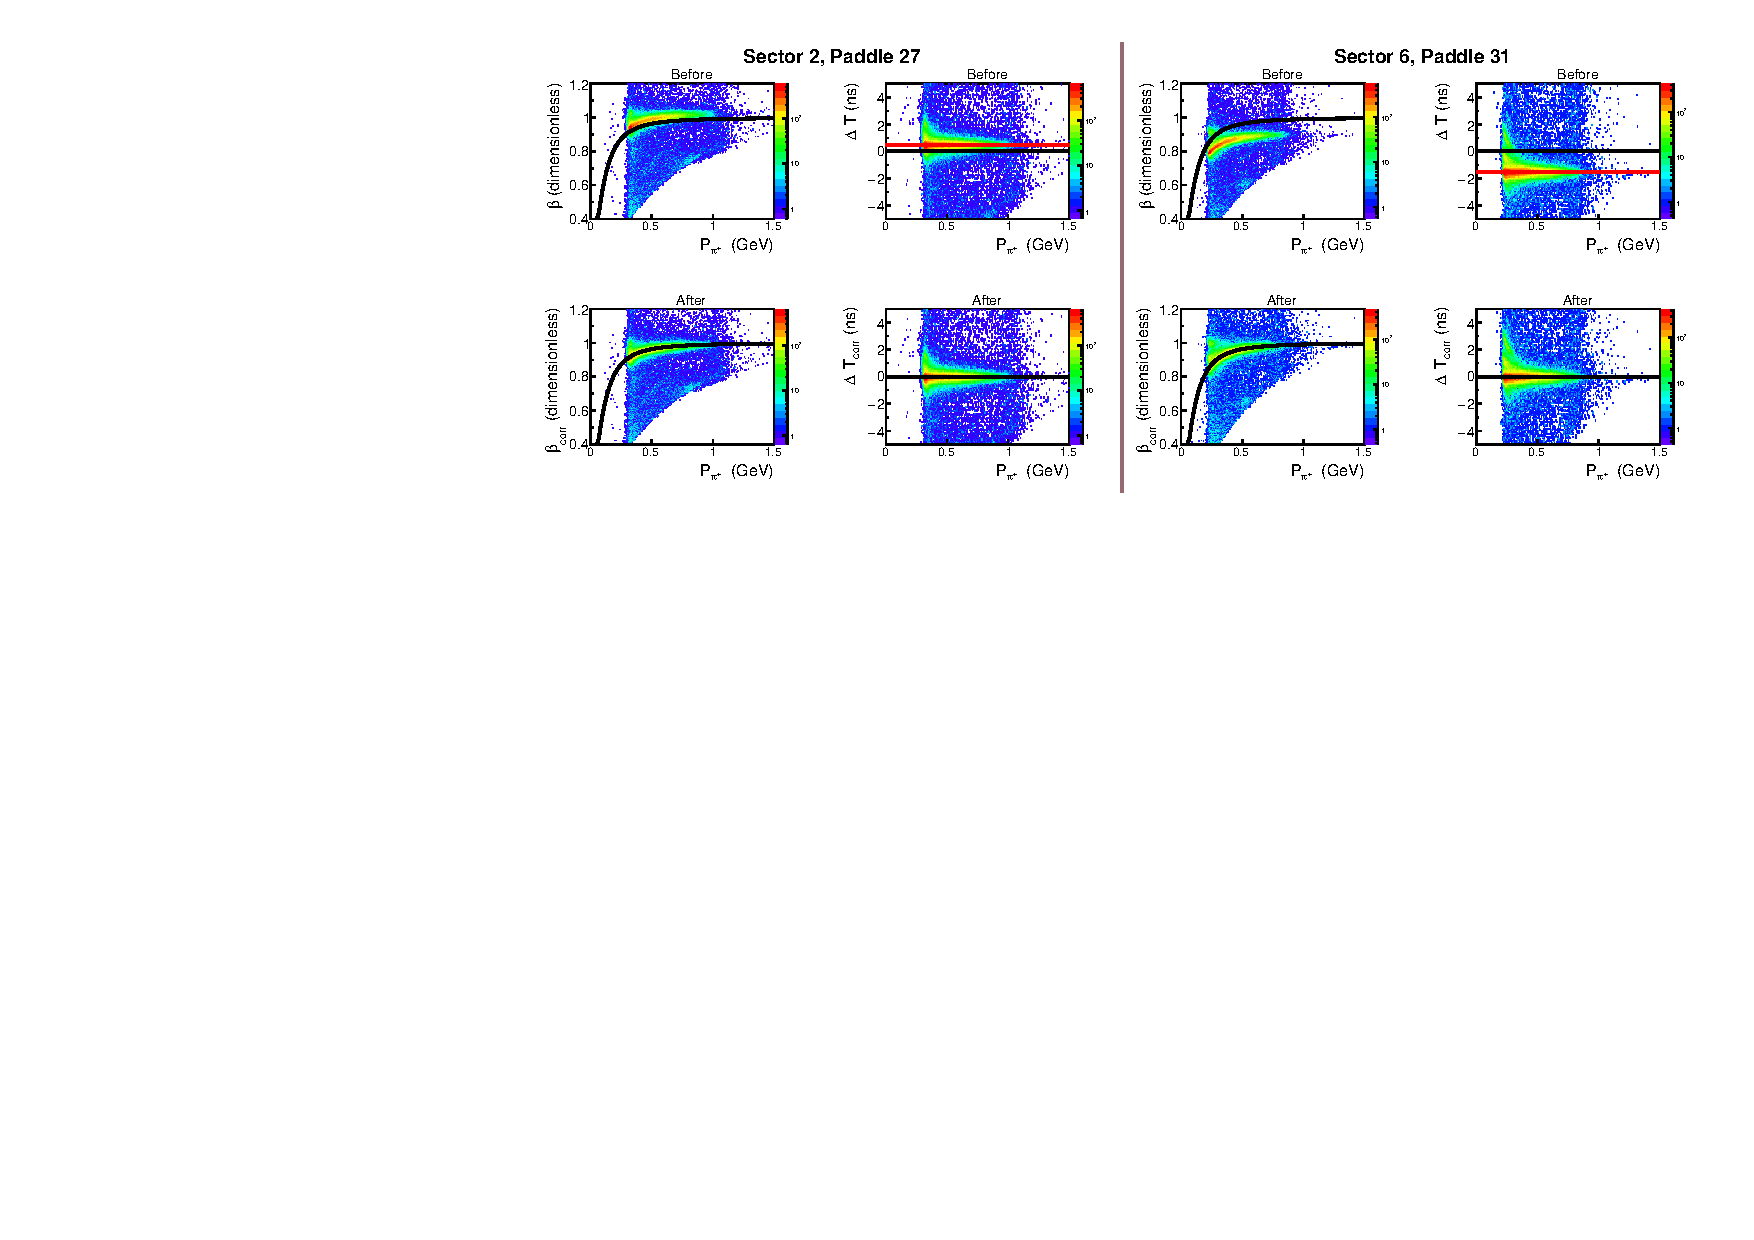
\includegraphics[width=\textwidth]{pictures/event_selection/hadron_id/shifted_paddles.pdf}}
\caption{\small Timing correction for type B problematic paddles \#27 in sector 2 (left side) and \#31 in sector 6 (right side) for $\pi^+$ candidates. The first column in each side shows the $\beta_{h}$ versus momentum distributions with the black curve corresponding to the nominal $\beta_{n}$ defined by Eq.~\eqref{eq:hadron_hadronmass}. The second column in each side corresponds to the $\Delta T$ versus momentum distributions, where the black horizontal line shows the position of zero and the red line shows the position of shifted $\Delta T$-band. The uncorrected distributions are given in the first row, while the influence of the correction is shown in the second row.  \label{fig:shifted_paddles}} 
\end{center}
\end{figure}


To cure the latter two types of problems, a so-called timing correction is developed. To perform this correction, the quantity $\Delta T$ is calculated, which corresponds to the time difference between the real TOF signal and the expected one.
\begin{equation}
\Delta T = \frac{l_{h}}{c}\left (\frac{1}{\beta_{n}} - \frac{1}{\beta_{h}}  \right ).
\label{eq:delta_t}
\end{equation}

%The quantity $\Delta T$ corresponds to the time difference between the real TOF signal and the expected one.
\looseness=-1
Figure~\ref{fig:shifted_paddles} illustrates the timing correction for type B problematic paddles \#27 in sector 2 (left side) and \#31 in sector 6 (right side) for $\pi^+$ candidates. The plots in the first row correspond to the $\beta_{h}$ versus momentum and $\Delta T$ versus momentum distributions before the correction. It is seen that $\beta_{h}$ versus momentum bands are shifted from their expected position shown by the black curve, which corresponds to the nominal $\beta_{n}$ defined by Eq.~\eqref{eq:hadron_hadronmass}. These shifts of $\beta_{h}$ versus momentum bands are caused by the corresponding shifts of the $\Delta T$ versus momentum bands from zero position shown by the black horizontal lines. The idea of the timing correction is to move $\Delta T$ bands back to the position around zero, as shown in the corrected $\Delta T$ versus momentum plots in the second row. The corrected value of $\beta$ is then calculated as
\begin{equation}
\beta_{corr} = \frac{1}{\frac{1}{\beta_{n}} - \frac{(\Delta T-t_{shift})\cdot c}{l_{h}}},
\label{eq:beta_corr}
\end{equation}
where $t_{shift}$ is the position of shifted $\Delta T$-band shown by the corresponding red horizontal line in Fig.~\ref{fig:shifted_paddles}.

The $\beta_{corr}$ versus momentum distributions are shown in second row in Fig.~\ref{fig:shifted_paddles}. As seen in these plots, $\beta_{corr}$ versus momentum bands demonstrate no shift from the black curves after the timing correction is applied.


\begin{figure}[htp]
\begin{center}
\framebox{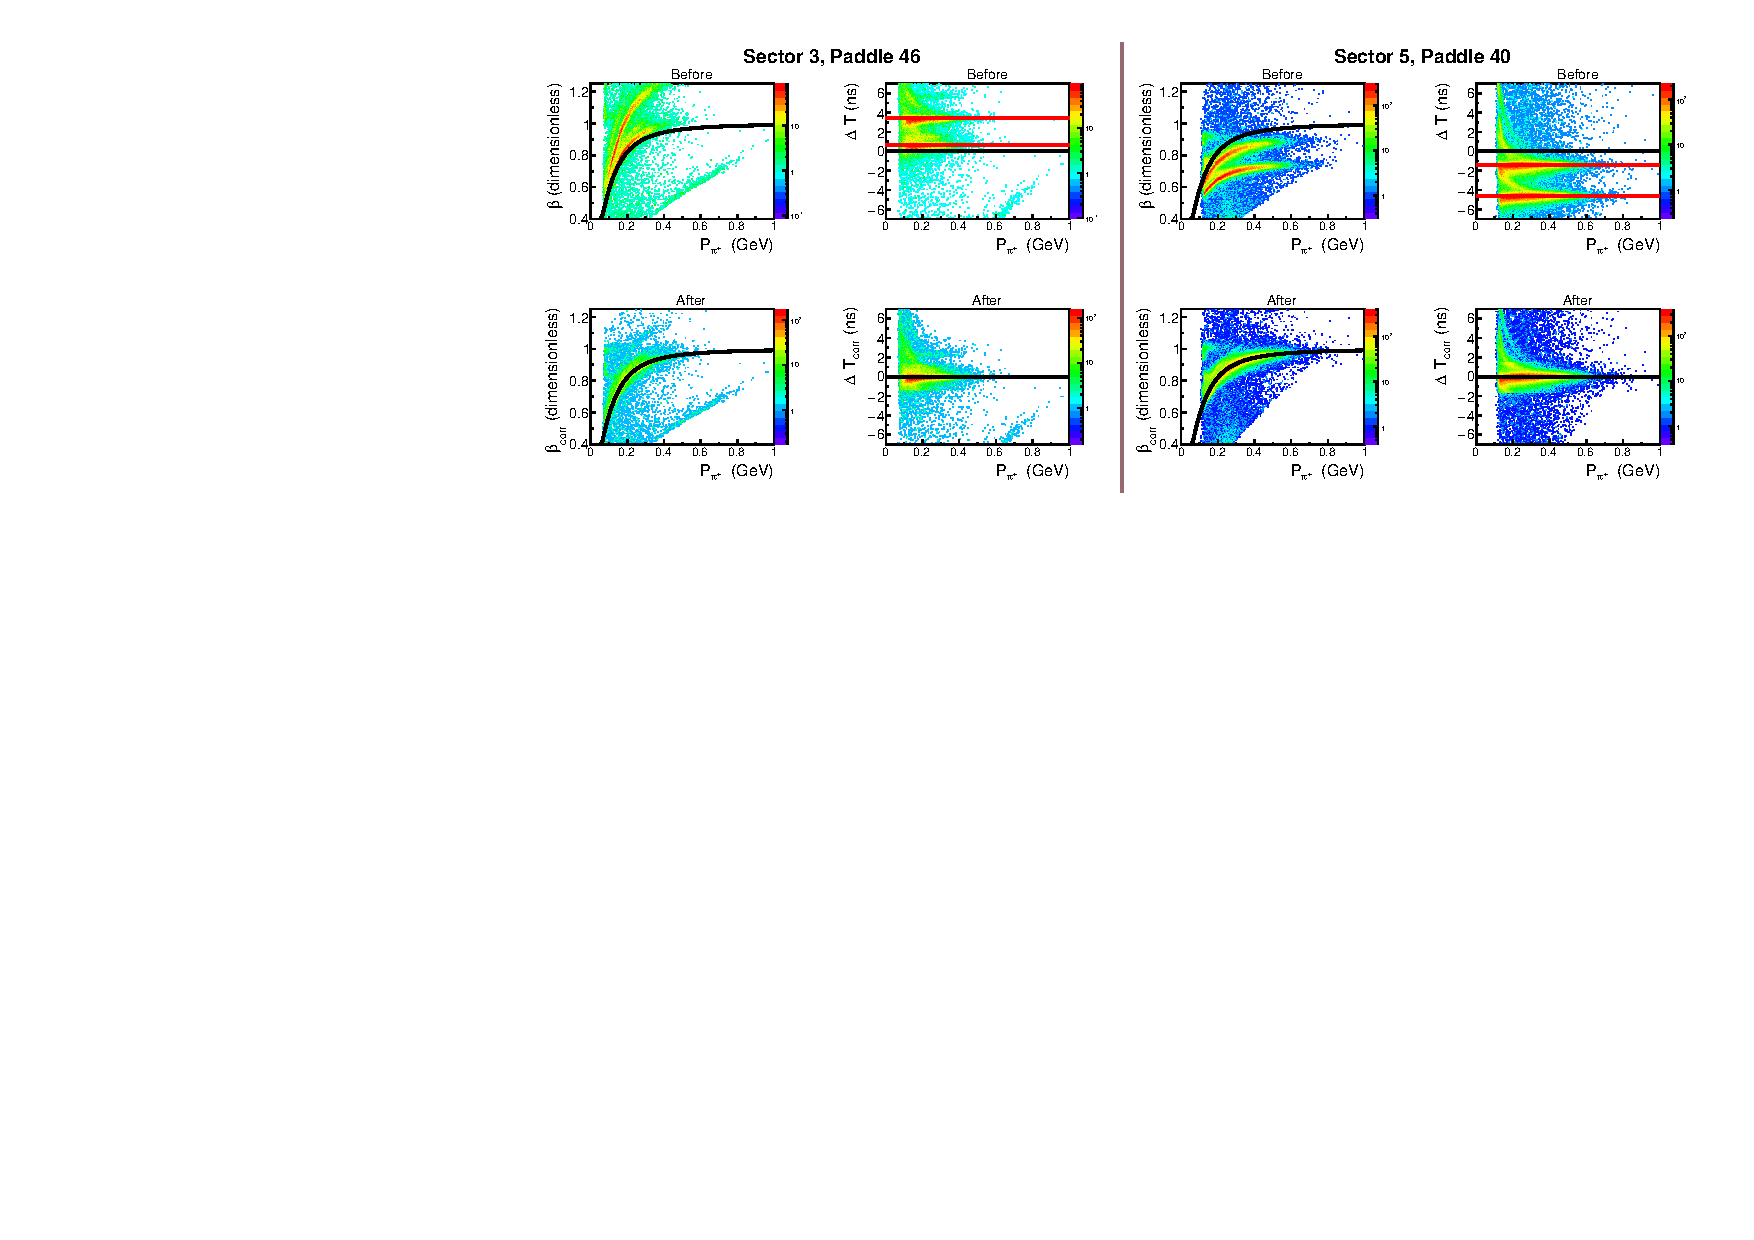
\includegraphics[width=\textwidth]{pictures/event_selection/hadron_id/double_paddles.pdf}}
\caption{\small Timing correction for type C problematic paddles \#46 in sector 3 (left side) and \#40 in sector 5 (right side) for $\pi^+$ candidates. The first column in each side shows the $\beta_{h}$ versus momentum distributions with the black curve corresponding to the nominal $\beta_{n}$ defined by Eq.~\eqref{eq:hadron_hadronmass}. The second column in each side corresponds to the $\Delta T$ versus momentum distributions, where the black horizontal line shows the position of zero and the red lines show the position of shifted $\Delta T$-bands. The uncorrected distributions are given in the first row, while the influence of the correction is shown in the second row. \label{fig:double_paddles}} 
\end{center}
\end{figure}

\begin{figure}[htp]
\begin{center}
\framebox{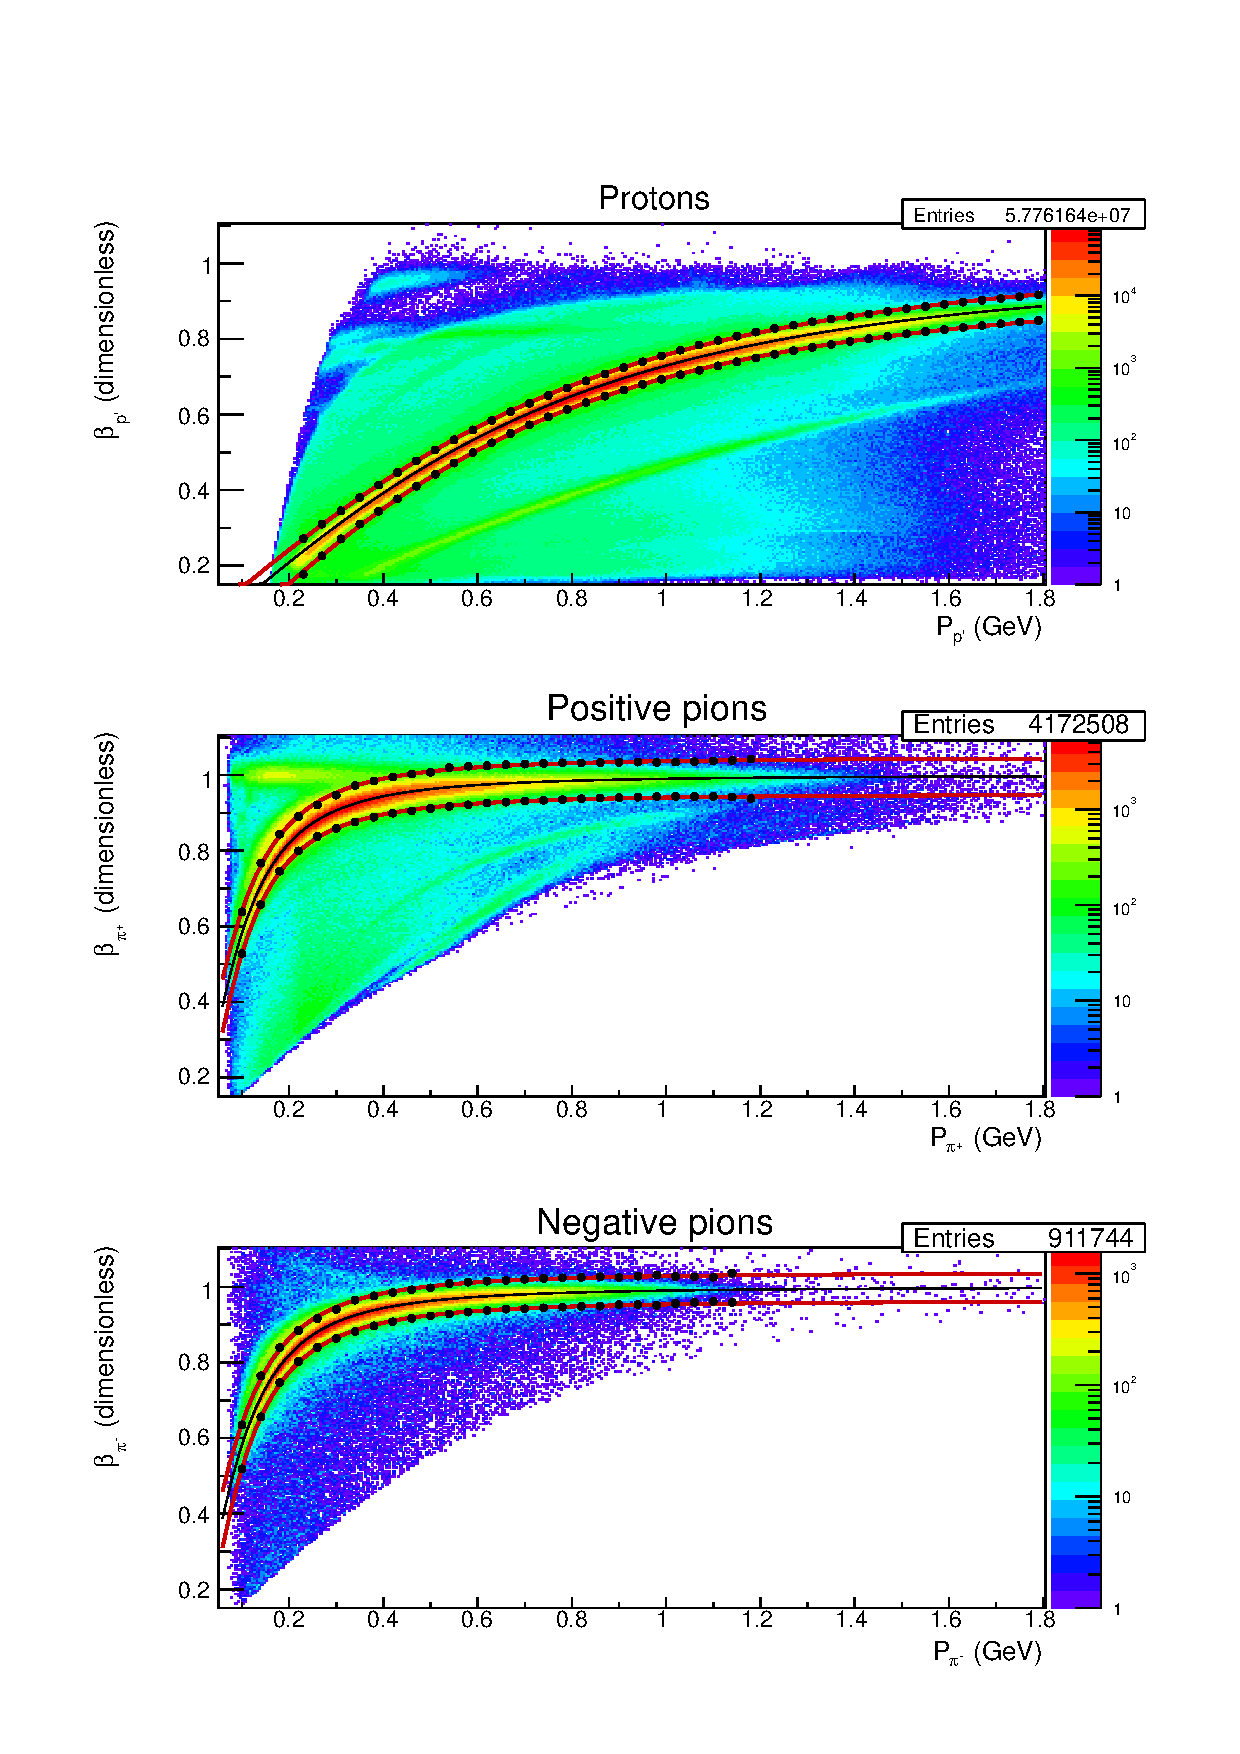
\includegraphics[width=14cm]{pictures/event_selection/hadron_id/hadron_id_cuts.pdf}}
\caption{\small $\beta_{corr}$ versus momentum distributions for proton (upper plot), positive pion (middle plot), and negative pion (bottom plot) candidates. Thin black solid curves in the middle of each band correspond to the nominal $\beta_{n}$ given by Eq.~\eqref{eq:hadron_hadronmass}. Black points correspond to the positions of Gaussian fit maxima $\pm 3\sigma$ for individual x-slices of the 2D histograms. These points are fit by the function Eq.~\eqref{eq:fit_f}, the resulting functions are shown by the red curves. Events between the red curves are selected for further analysis. \label{fig:hadron_id}} 
\end{center}
\end{figure}

Figure~\ref{fig:double_paddles} illustrates the timing correction for type C problematic paddles \#46 in sector 3 (left side) and \#40 in sector 5 (right side) for $\pi^+$ candidates. The plots in the first row clearly show the double band structures in $\beta_{h}$ versus momentum and $\Delta T$ versus momentum distributions. To perform timing correction for this type of paddles, one needs to determine the position $t_{shift}$ of each incorrect $\Delta T$-band (see horizontal red lines in Fig.~\ref{fig:double_paddles}) and then to move both of them to the correct position around zero, as demonstrated in the second row. The corrected value of $\beta$ is again calculated according to Eq.~\eqref{eq:beta_corr} with the only distinction, that events from different $\Delta T$-bands are treated separately and different $t_{shift}$ values are used for them.

The $\beta_{corr}$ versus momentum distributions are shown in the second row in Fig.~\ref{fig:double_paddles}. As seen in these plots, after the timing correction is applied $\beta_{corr}$ versus momentum bands demonstrate neither double band structures nor shifts from the black curves.


Figures~\ref{fig:shifted_paddles} and~\ref{fig:double_paddles} give examples of the timing correction for $\pi^+$ candidates. Similar corrections have also been performed for proton and $\pi^{-}$ candidates.


After the timing problems are eliminated in each TOF paddle, the hadron identification can be made. For the hadron identification, only events with good electron candidates that have been selected in the previous step are used. Figure~\ref{fig:hadron_id} shows $\beta_{corr}$ versus momentum distributions for each type of hadron candidate: protons (upper plot), positive pions (middle plot), and negative pions (bottom plot). These distributions include all sectors and all TOF paddles (with the exclusion of bad ones). The red curves show the corresponding hadron id cuts. These curves were obtained in the following way. Firstly, x-slices of the 2D histograms are fit by Gaussians. In this way points that correspond to the positions of the fit maxima $\pm 3\sigma$ are obtained. These points are shown by black bullets in Fig.~\ref{fig:hadron_id}. They determine the upper and lower boundaries for the cut\footnote[5]{Note that to establish the upper cut boundary for pions, the $3\sigma$ value was used only for $p_{\pi}>0.54$~GeV. For $p_{\pi}<0.54$~GeV different smaller values were used in order to better separate pions from the small upper band, which is thought to correspond to muons.}. Finally, to obtain smooth curves, all points are fit by the following function,
\begin{equation}
f(p_{h})=\frac{a_{0}\cdot p_{h}}{\sqrt{a_{1}\cdot p_{h}^{2}+m_{h}^{2}+a_{2}}}+a_{3},
\label{eq:fit_f}
\end{equation}
where $p_{h}$ is the hadron momentum, $m_{h}$ hadron mass, and $a_{0}$, $a_{1}$, $a_{2}$, $a_{3}$ fit parameters.

Events which are located between the red curves in Fig.~\ref{fig:hadron_id} are selected for further analysis and treated as good corresponding hadron candidates. It also needs to be mentioned that the distribution for positive pions was plotted only for events that already have a good proton candidate, and the distribution for negative pions was plotted only for events with good proton and positive pion candidates. Furthermore, in order to simplify the analysis process, all hadrons were preselected on an initial analysis step. The consequence of this preselection is the fact that distributions shown in Fig.~\ref{fig:hadron_id} contain areas that are not populated with events.

The hadron identification cuts established in this way are applied to the reconstructed Monte Carlo events as well. 



\section{Momentum corrections}
\label{Sect:momcorr}

\subsection{Proton momentum correction (energy loss)}
\label{Sect:pr_en_loss}


While traveling through the detector and the target, the final state particles lose a part of their energy due to the interactions with the medium. Therefore, the measured particle momentum appears to be lower than the actual value. GSIM simulation of the CLAS detector correctly propagates particles  through the media and, therefore, the effect of the energy loss is included into the efficiency and does not impact the extracted cross sections. However, in order to avoid shifts in the distributions of some kinematic quantities (e.g. missing masses) from their expected values, an energy loss correction is applied to the proton momentum magnitude, since the low-energy protons are affected the most by energy loss in the materials. This correction is based on the GSIM simulation of the CLAS detector and is performed for both experimental and reconstructed Monte Carlo events.

\begin{figure}[htp]
\begin{center}
\framebox{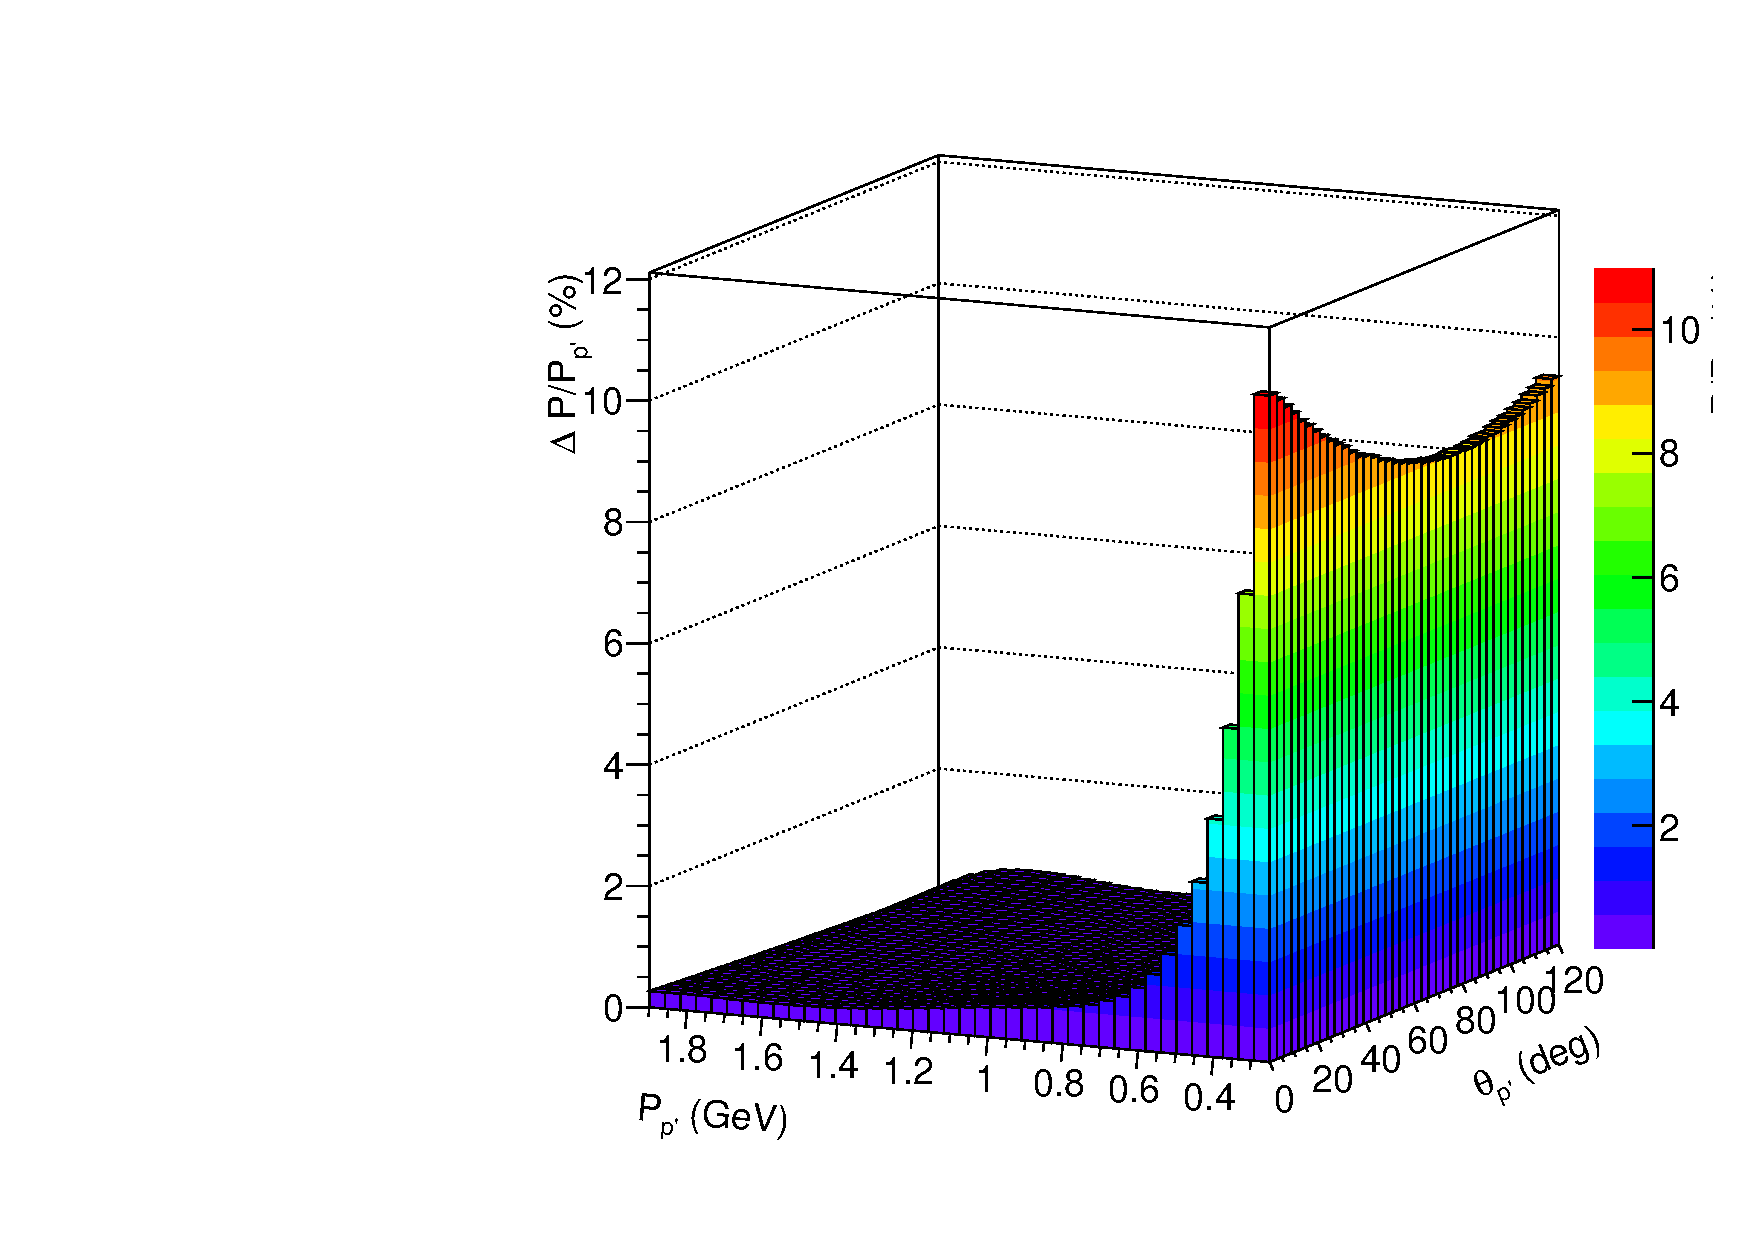
\includegraphics[width=9cm]{pictures/event_selection/mom_corr/eloss2d.pdf}}
\caption{\small Percentage of momentum that protons lose when they move through the detector and target media as a function of the momentum $P_{p'}$ and scattered angle $\theta_{p'}$ of the final proton. \label{fig:eloss}} 
\end{center}
\end{figure}

To obtain the correction function, the quantity $\Delta P$ that is the difference between the generated and reconstructed proton momenta was considered. This quantity was binned in the reconstructed proton momentum $P_{p'}$ and polar angle $\theta_{p'}$ and fit by a Gaussian in each $(P_{p'},~\theta_{p'})$ bin. The obtained mean values were further fit by a fifth order polynomial as a function of $P_{p'}$ in each $\theta_{p'}$ bin. Then the parameters of the resulting fit functions were fit as a function of $\theta_{p'}$ by a second order polynomial. 



The resulting energy loss correction function is shown in Fig.~\ref{fig:eloss}. It gives the percentage of the momentum that protons lose when they move through the detector and target media. 

Note that if one wants to isolate the pure effect of the energy loss, the difference between proton momenta for events reconstructed with and without detector and target materials must be considered. Since in the applied procedure the difference between generated and reconstructed proton momenta is analyzed, the correction function shown in Fig.~\ref{fig:eloss} can also include other effects that lead to improper proton momentum reconstruction.



\subsection{Electron momentum correction}
\label{Sect:el_momcor}

Due to slight misalignments in the DC position, small inaccuracies in the description of the torus magnetic field, and other possible reasons the momentum and angle of particles may have some small systematic deviations from their real values. These effects being of undefined origin cannot be simulated in GSIM, therefore a special momentum correction procedure is needed for the experimental data. According to~\cite{KPark:momcorr}, the evidence of the need for such corrections is most directly seen in the dependence of the elastic peak position on the azimuthal angle of the scattered electrons. It is shown in~\cite{KPark:momcorr} that the elastic peak position is shifted from the true value (0.938 GeV) and this shift is sector dependent.  

The significance of this effect depends on the beam energy. In the analysis~\cite{Fed_an_note:2017} it is shown that a beam energy of 2.039 GeV leads to the small shift ($\sim$ 3 MeV) in elastic peak position, while the study~\cite{KPark:momcorr} demonstrates that in case of  5.754 GeV beam energy this shift reaches 20 MeV. Moreover, the study~\cite{KPark:momcorr} also shows that this effect becomes discernible only if the particle momentum is sufficiently high (e.g. for pions the correction is needed only if their momentum is higher than 2 GeV). Thus, the small beam energy of this analyzed dataset and the fact that in double-pion kinematics hadrons carry only a small portion of the total momentum allows us to come to the conclusion that the correction is needed only for electrons, while deviation in hadron momenta can be neglected.

\begin{figure}[htp]
\begin{center}
\framebox{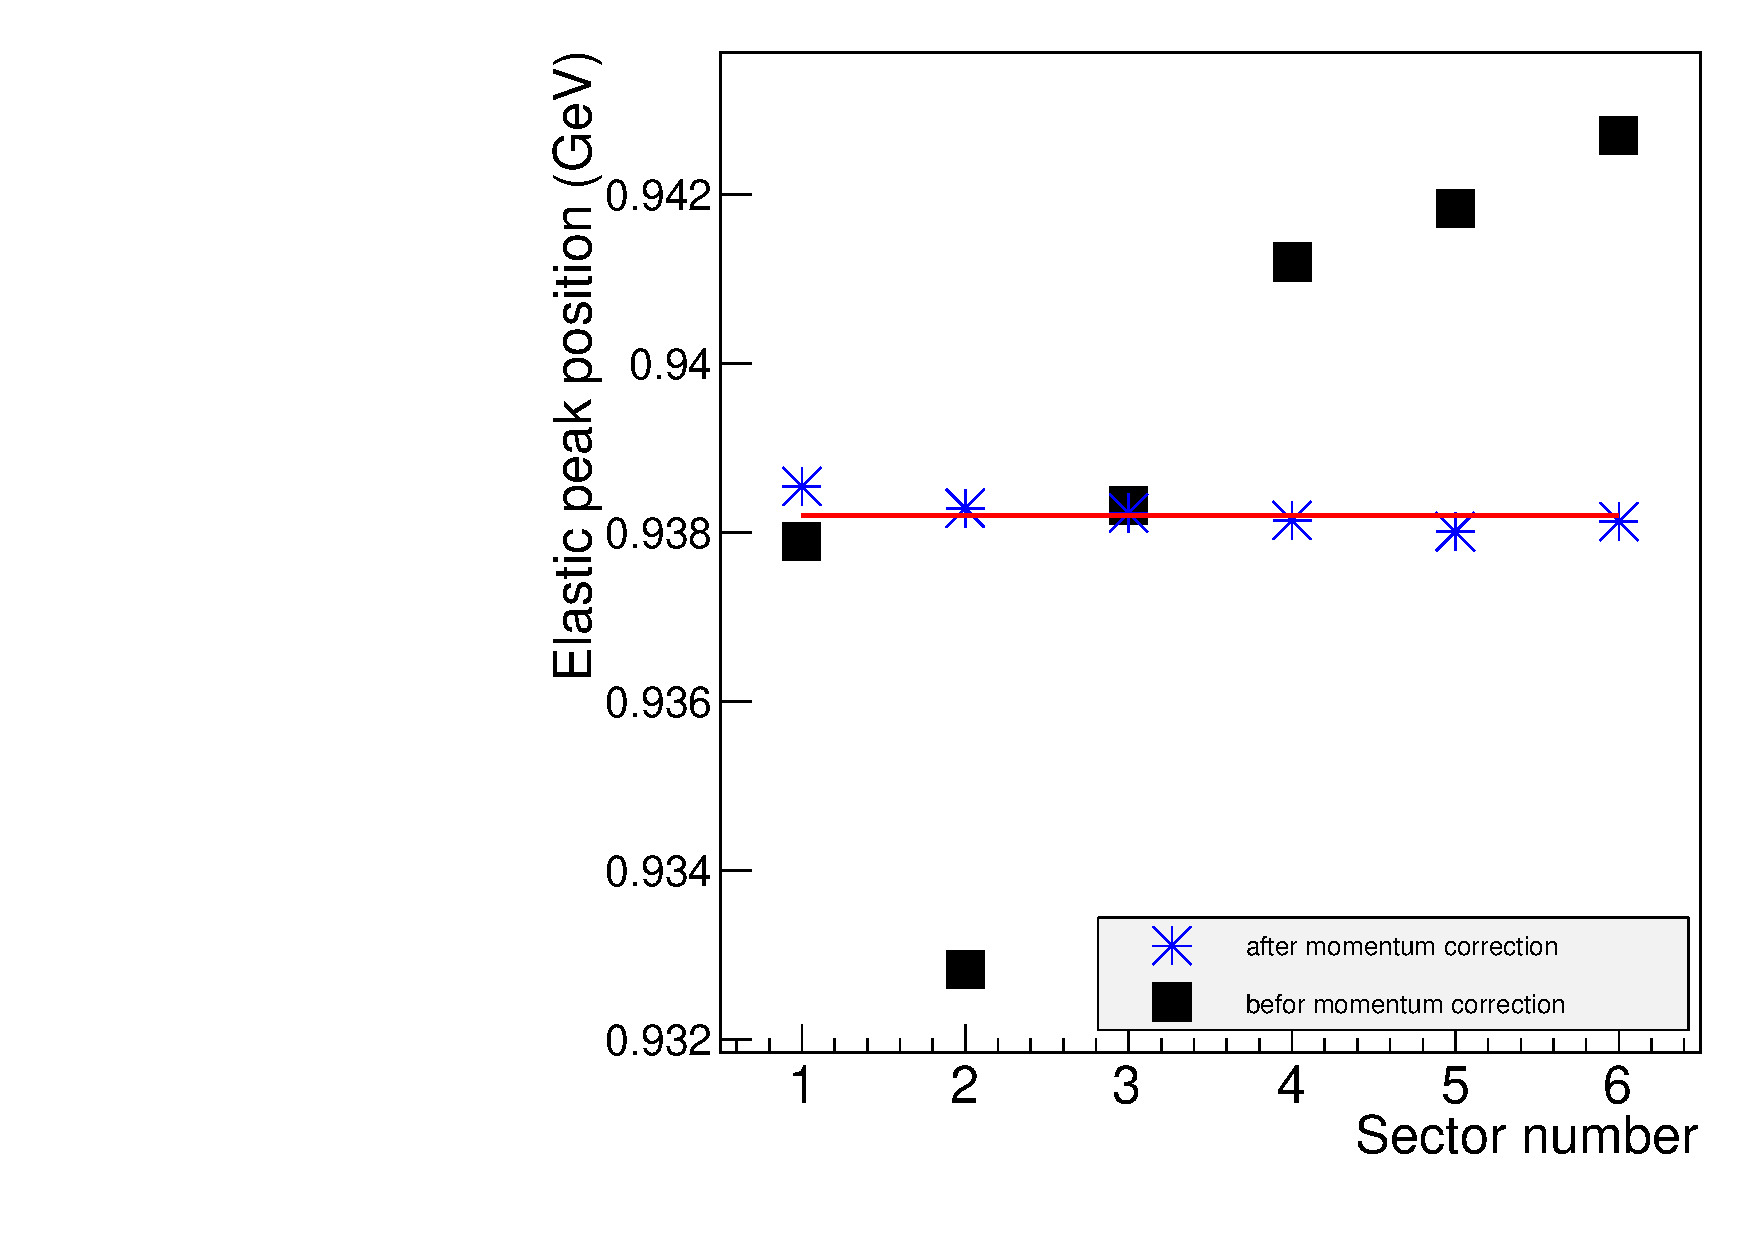
\includegraphics[width=8cm]{pictures/event_selection/mom_corr/elast_pic_position.pdf}}
\caption{\small Elastic peak position for the six CLAS sectors before (black squares) and after (blue stars) electron momentum correction for the proton part of ``e1e" dataset. The horizontal red line shows the proton mass. This figure is taken from the analysis~\cite{Fed_an_note:2017}. \label{fig:el_mom_corr_peak_position}} 
\end{center}
\end{figure}

Since this analysis suffers from additional complications as binding and motion of the target proton inside the deuteron, it was considered sensible to use the electron momentum corrections that have previously been developed and tested in the analysis of the free proton part of ``e1e" dataset at the same beam energy~\cite{Fed_an_note:2017}. To establish them, the approach~\cite{KPark:momcorr}, which is based on elastic kinematics, was used. These corrections include electron momentum magnitude correction as well as electron polar angle correction, which were developed for each CLAS sector individually.  


Figure~\ref{fig:el_mom_corr_peak_position}, which was taken from the analysis~\cite{Fed_an_note:2017}, demonstrates that after the electron momentum corrections the elastic peak position for all CLAS sectors gets closer to the proton mass, shown by the red horizontal line.

\begin{figure}[htp]
\begin{center}
\framebox{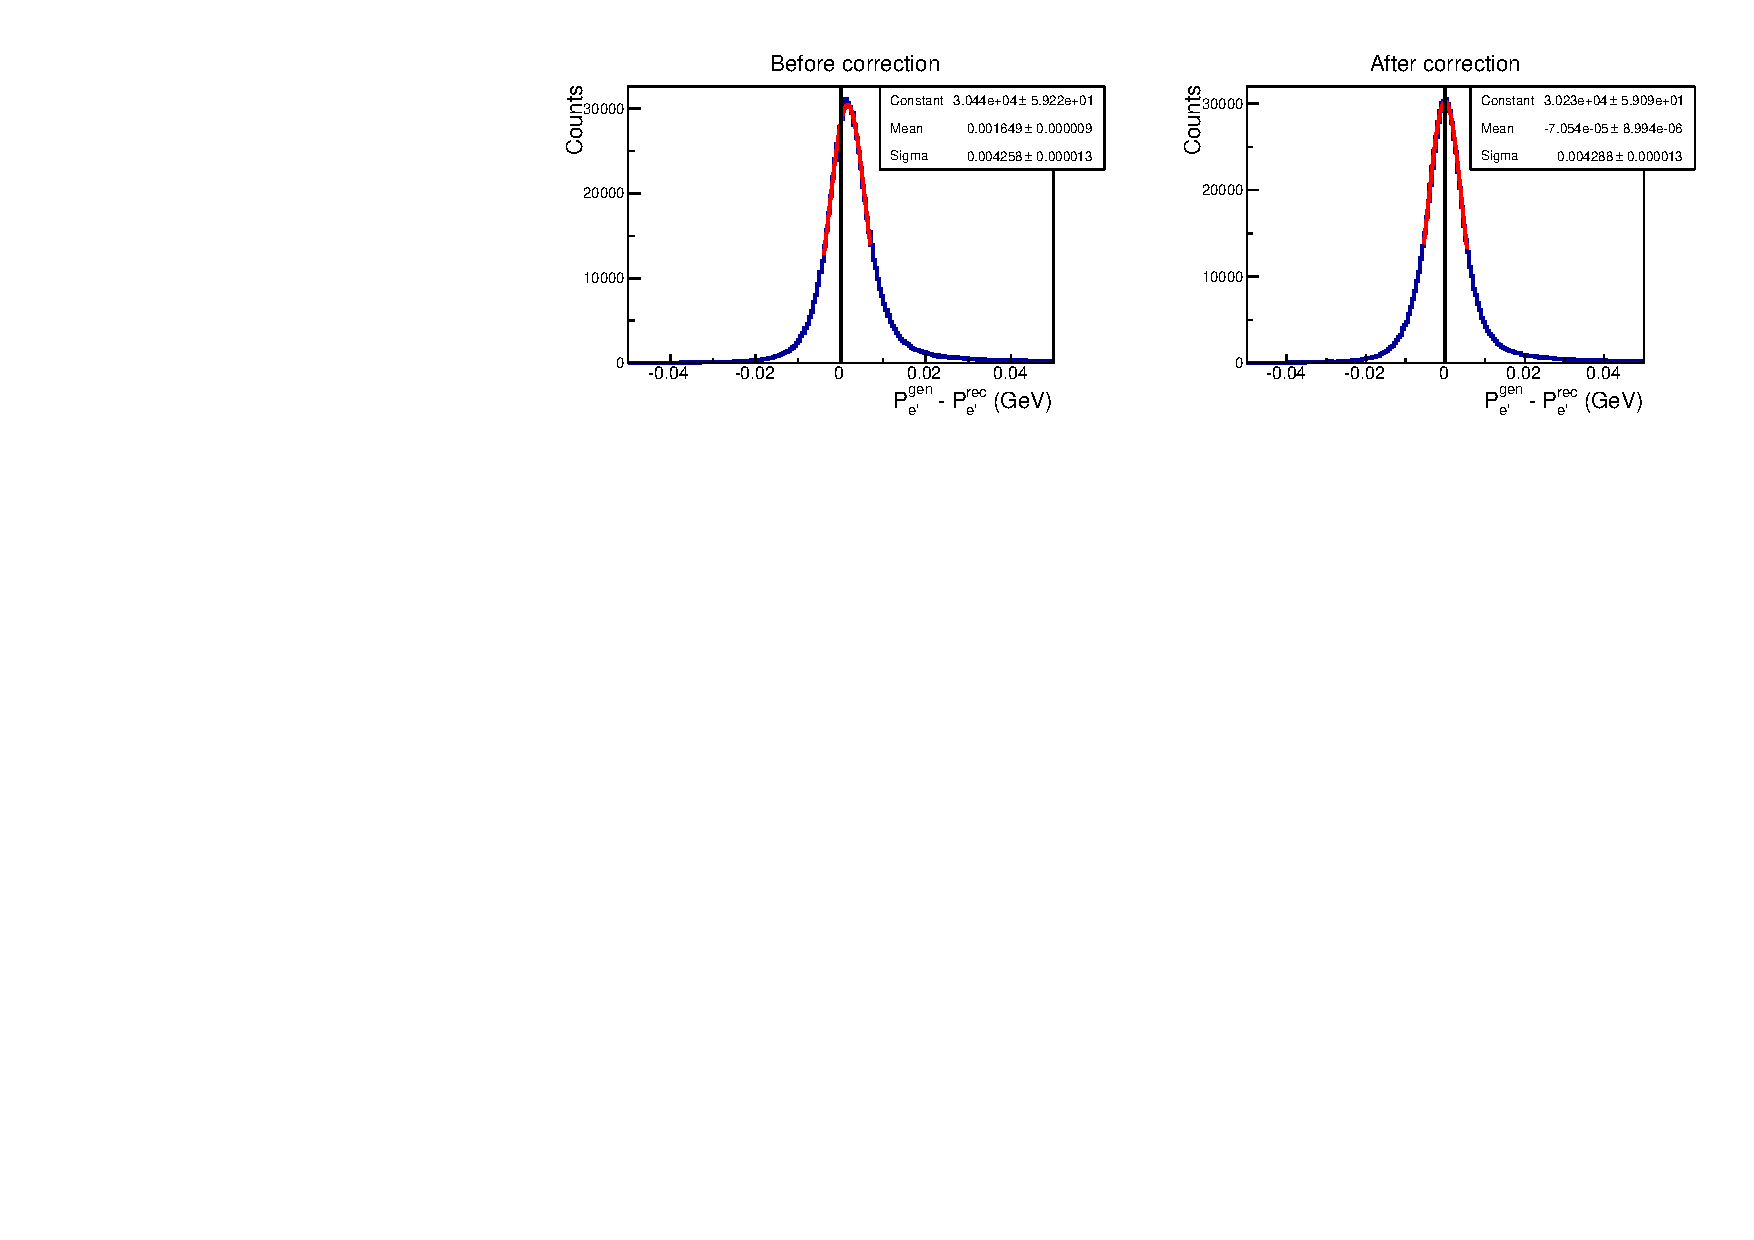
\includegraphics[width=14cm]{pictures/event_selection/mom_corr/el_sim_momcor_bef_aft.pdf}}
\caption{\small Difference between generated and reconstructed electron momenta before (left plot) and after (right plot) the correction of the momentum magnitude, which has been applied to the reconstructed electrons. The vertical black line shows the position of zero. \label{fig:el_mom_corr_sim}} 
\end{center}
\end{figure}

The correction discussed above is applied only for experimental data. As for the Monte Carlo simulation, it turns out that due to unknown reasons (most likely because electrons lose some energy when they travel through the detector and target media) the reconstructed electron momentum appears to be slightly lower than the generated one. This effect is demonstrated in the left plot of Fig.~\ref{fig:el_mom_corr_sim}, where the event distribution of the quantity $\Delta P$ (which is the difference between generated and reconstructed electron momenta) is presented. Therefore, an adapted procedure of correcting the electron momentum magnitude is also applied to the reconstructed Monte Carlo events. This procedure is similar to that used for the proton energy loss (see Sect.~\ref{Sect:pr_en_loss}). The correction depends only on the scattered electron momentum and polar angle, but not on the CLAS sector. The typical value of this correction is 0.2\%. The right plot in Fig.~\ref{fig:el_mom_corr_sim} shows the result of the correction. As seen in this plot, the mean value of the quantity $\Delta P$ demonstrates no shift from zero when the momentum magnitude for reconstructed electron is corrected. 

